\documentclass[11pt]{article}
\usepackage{graphicx}
\usepackage{hyperref}
%\usepackage{appendix}
\usepackage{amsmath}
\usepackage{amsthm}
\usepackage{amssymb}
\usepackage{float}
\usepackage{commath}
\usepackage{booktabs}
\renewcommand{\arraystretch}{1.2}
\usepackage{siunitx}
\sisetup{detect-all}
\usepackage{listings}
\usepackage{color} %red, green, blue, yellow, cyan, magenta, black, white
\definecolor{mygreen}{RGB}{28,172,0} % color values Red, Green, Blue
\definecolor{mylilas}{RGB}{170,55,241}
\usepackage[a4paper,margin=20mm]{geometry}
\numberwithin{equation}{section}
\setlength{\parskip}{\baselineskip}
\setlength{\parindent}{0pt}
\hypersetup{
    colorlinks=true,
    linkcolor=black,
    filecolor=black,      
    urlcolor=black,
    citecolor=black
}
\urlstyle{same}
\begin{document}
\title{\textbf{UCL Mechanical Engineering 2020/2021}\\MECH0013 Final Assessment}
\author{NCWT3}
\maketitle
\tableofcontents
\listoffigures
\section{Question 1}
\subsection{i}
Straight section analysis:
\begin{figure}[H]
    \centering
    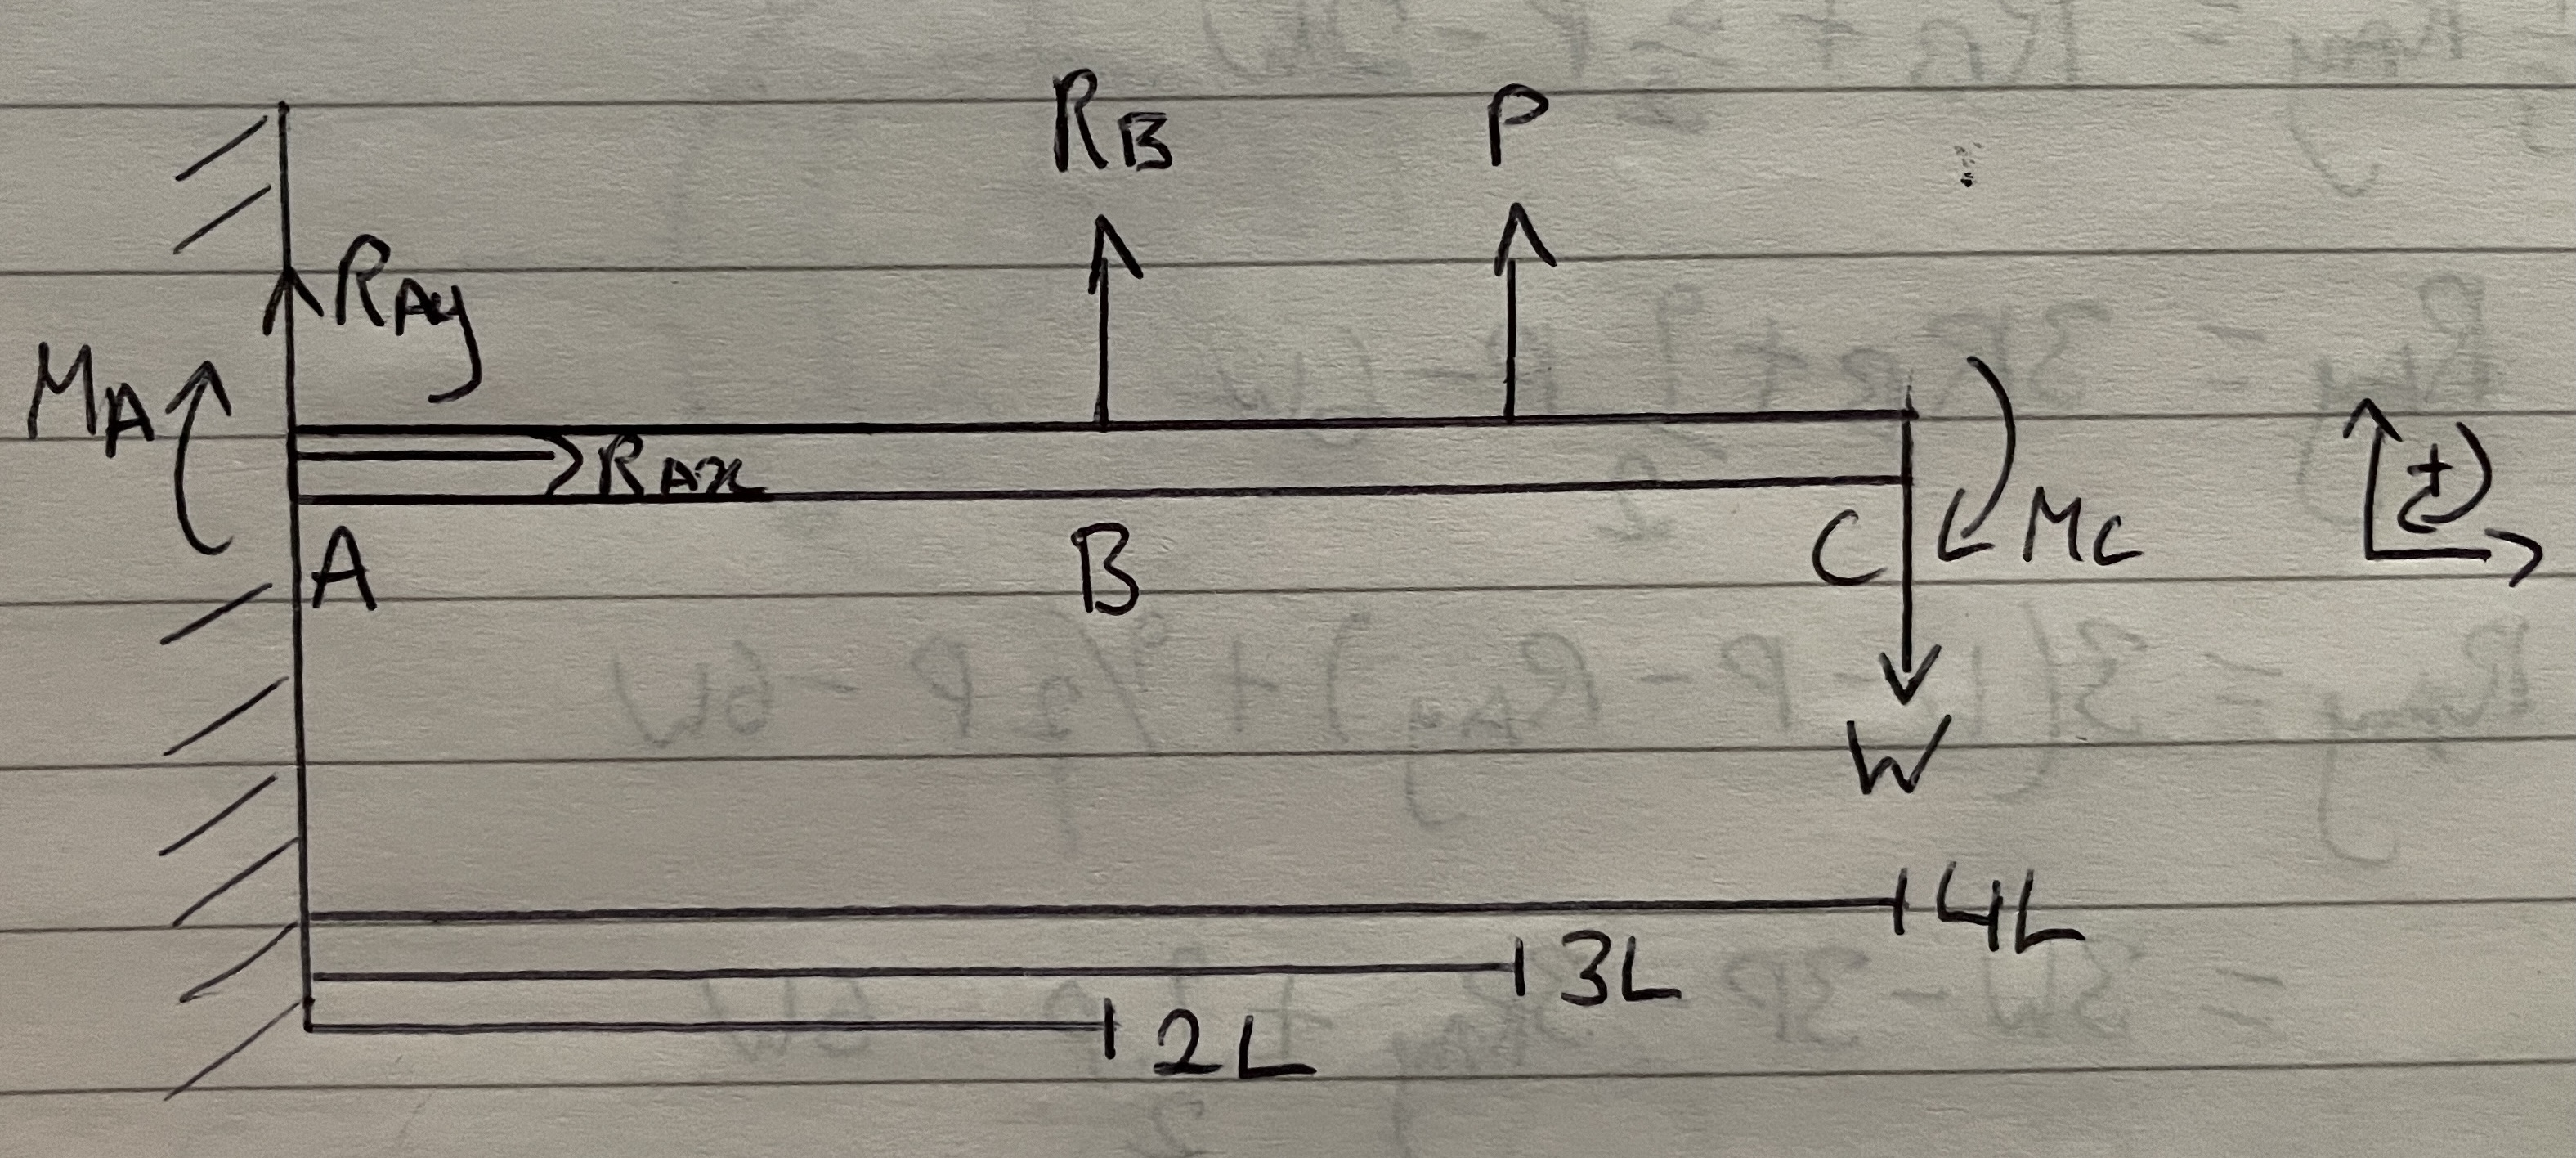
\includegraphics[width = 0.75\textwidth]{./img/q1i.jpg}
    \caption{Diagram to show horizontal beam arrangement.}
    \label{fig:q1i}
\end{figure}
Equilibrium conditions:
\begin{align}
    \sum F_x: \; &R_{Ax} = 0\\
    \sum F_y: \; &R_{Ay} + R_B + P = W \label{q1isumy}\\
    \sum M_A: \; &M_A + M_C + 4WL = 2R_B L + 3PL \label{q1isumM}
\end{align}
Using Macaulay's method:
\begin{align}
    M &= M_A + R_{Ay}x + R_B <x- 2L> + P<x-3L> \label{eq:q1i1}
\end{align}
Slope:
\begin{align}
    \theta &= \frac{1}{EI} \int \left(M\right)\dif x\\
    \theta &= \frac{1}{EI} \int \left(M_A + R_{Ay}x + R_B <x- 2L> + P<x-3L>\right) \dif x\\
    \theta &= \frac{1}{EI} \left[M_A x + \frac{R_{Ay}x^2}{2} + \frac{R_b<x - 2L>^2}{2} + \frac{P<x-3L>^2}{2}\right] + \theta_0
\end{align}
Deflection:
\begin{align}
    y &= \int \left(\theta\right) \dif x\\
    y &= \int \left(\frac{1}{EI} \left[M_A x + \frac{R_{Ay}x^2}{2} + \frac{R_b<x - 2L>^2}{2} + \frac{P<x-3L>^2}{2}\right] + \theta_0\right) \dif x\\
    y &= \frac{1}{EI} \left[\frac{M_A x^2}{2} + \frac{R_{Ay}x^3}{6} + \frac{R_B<x- 2L>^3}{6} + \frac{P<x-3L>^3}{6}\right] + \theta_0 x +y_0 \label{eq:slope}
\end{align}
Curved section analysis:
\begin{figure}[H]
    \centering
    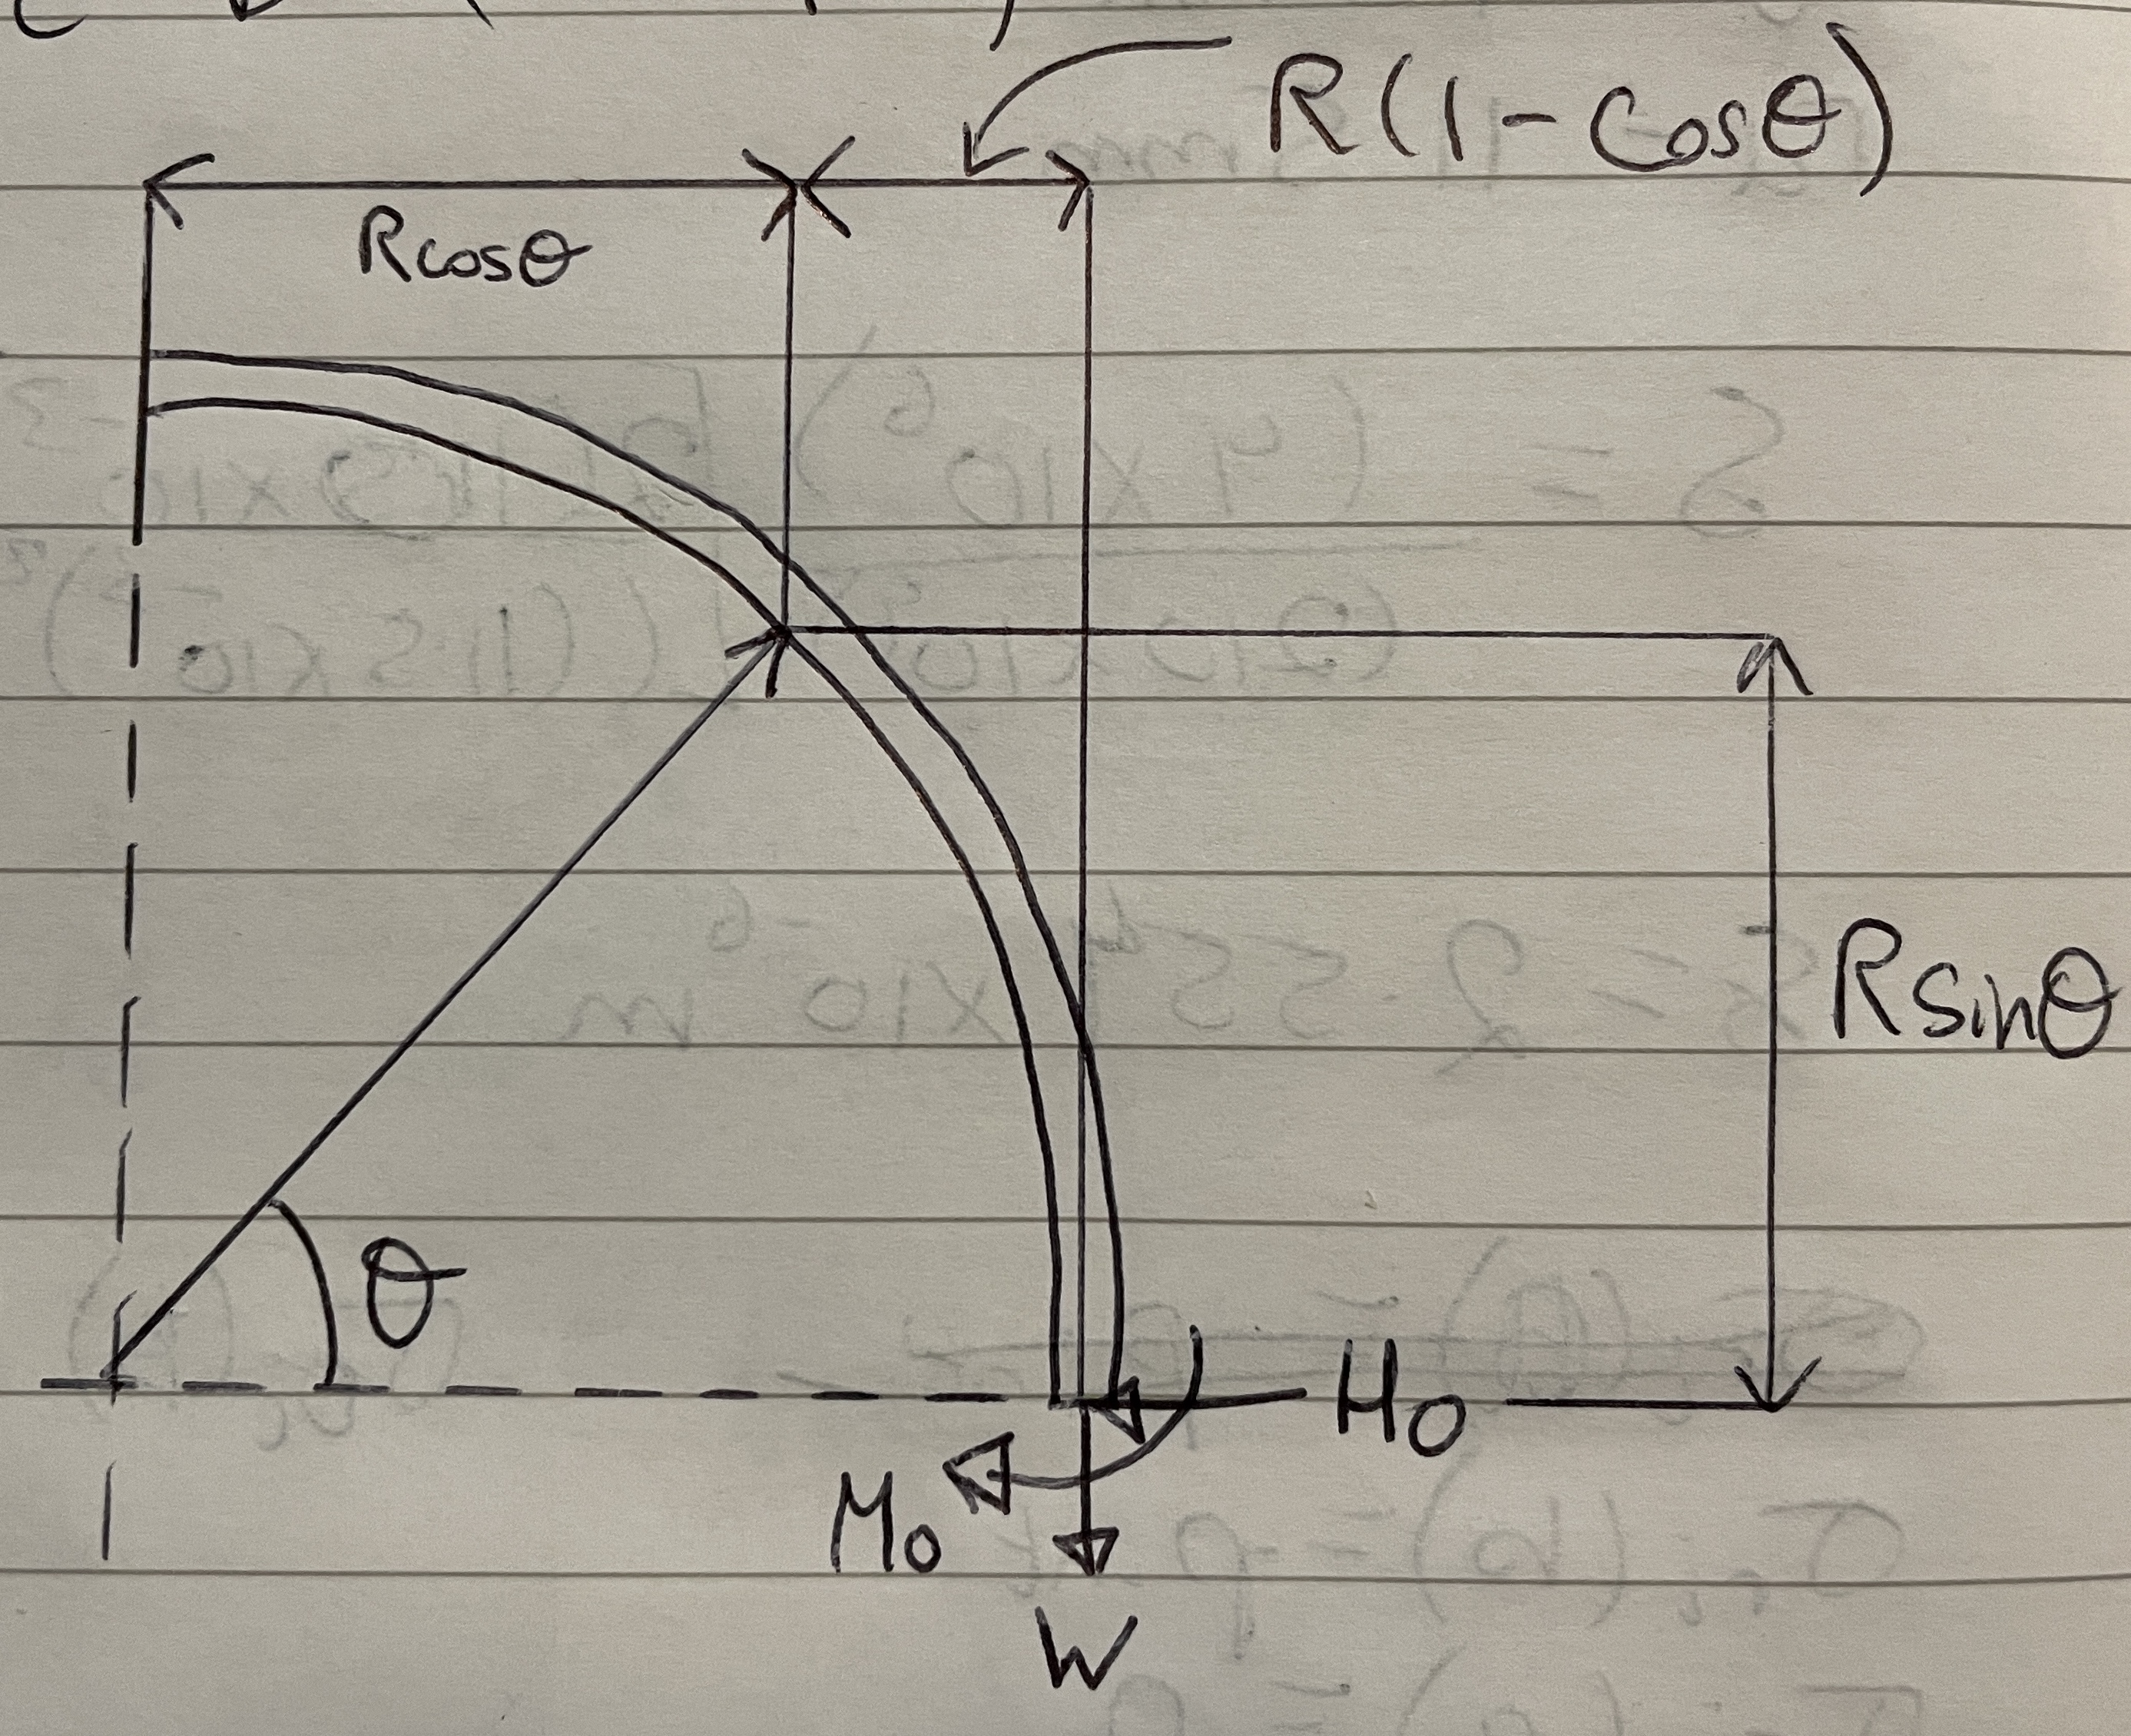
\includegraphics[height = 5cm]{./img/q1ii.jpg}
    \caption{Diagram to show curved beam arrangement.}
    \label{fig:q1ii}
\end{figure}
\begin{align}
    M(\theta) &= WR\left(1 - \cos \theta\right) + H_0 R \sin\theta + M_0\\
    \frac{\partial M}{\partial M_0} &= 1\\
    \varphi_A &= \int_0^L \left(\frac{M}{EI}\frac{\partial M}{\partial M_0}\right)\dif x = 0
\end{align}
Converting to polar ($\dif x = R \dif \theta$):
\begin{align}
    \varphi = \frac{1}{EI}\int_0^{\frac{\pi}{2}} \left( \left(WR \left(1-\cos \theta\right)+H_0 R\sin\theta + M_0 \right)\left(1\right)\left(R\right) \right)\dif \theta
\end{align}
$M_0$ and $H_0$ represent dummy loads and can be neglected:
\begin{align}
    \varphi &= \frac{1}{EI}\int_0^{\frac{\pi}{2}} \left(WR^2\left(1-\cos\theta\right)\right)\dif \theta\\
    \varphi &= \frac{1}{EI} \left[WR^2\left(\theta-\sin\theta\right)\right]^{\frac{\pi}{2}}_0\\
    \varphi &= \frac{WR^2\left(\frac{\pi}{2}-1\right)}{EI}
\end{align}
Boundary conditions:
\begin{gather}
    x = 0, \; y = 0 \therefore y_0 = 0\\
    x = 0, \; \theta = 0 \therefore \theta_0 = 0\\
    x = 2L, \; y = 0 \label{q1ibc3}\\
    x = 4l, \; \theta = \frac{WR^2\left(\frac{\pi}{2}-1\right)}{EI} \label{q1ibc4}
\end{gather}
From \ref{q1ibc3}:
\begin{align}
    0 &= \frac{1}{EI} \left[\frac{M_A\left(2L\right)^2}{2} + \frac{R_{Ay}\left(2L\right)^3}{6} + \frac{R_B <2L - 2L>^3}{6}\right]\\
    0 &= \frac{1}{EI} \left[2M_A L^2 + \frac{4R_{Ay}L^3}{3} + 0\right]\\
    0 &= 2M_AL^2 + \frac{4R_{Ay}L^3}{3}\\
    M_A &= \frac{-2R_{Ay}L}{3} \label{q1iMA}
\end{align}
From \ref{q1ibc4}:
\begin{align}
    \frac{WR^2\left(\frac{\pi}{2}-1\right)}{EI} &= \frac{1}{EI} \left[M_A \left(4L\right) + \frac{R_{Ay}\left(4L\right)^2}{2} + \frac{R_B<4L-2L>^2}{2} + \frac{P<4L-3L>^2}{2}\right]\\
    WR^2\left(\frac{\pi}{2}-1\right) &= 4M_A L + 8R_{Ay}L^2 + 2R_BL^2 + \frac{PL^2}{2}
\end{align}
Substituting \ref{q1iMA}:
\begin{align}
    WR^2\left(\frac{\pi}{2}-1\right) &= -\frac{8R_{Ay}L^2}{3} + 8R_{Ay}L^2 + 2R_BL^2 + \frac{PL^2}{2}\\
    WR^2\left(\frac{\pi}{2}-1\right) &= \frac{16R_{Ay}L^2}{3} + 2R_BL^2 + \frac{PL^2}{2}
\end{align}
From \ref{q1isumy}:
\begin{align}
    R_B = W - P - R_{Ay} \label{q1iRB}
\end{align}
Substituting \ref{q1iRB}:
\begin{align}
    WR^2\left(\frac{\pi}{2}-1\right) &= \frac{16R_{Ay}L^2}{3} + 2\left(W - P - R_A\right)L^2 + \frac{PL^2}{2}\\
    WR^2\left(\frac{\pi}{2}-1\right) &= \frac{16R_{Ay}L^2}{3} + 2WL^2 - 2PL^2 - 2R_AL^2 + \frac{PL^2}{2}\\
    WR^2\left(\frac{\pi}{2}-1\right) &= \frac{10R_{Ay}L^2}{3} + 2WL^2 -\frac{3PL^2}{2}
\end{align}
From \ref{q1isumM}, \ref{q1isumy}, \ref{q1iRB}, \ref{q1iMA}: 
\begin{align}
    -\frac{2R_{Ay}L}{3} + WR + 4WL &= 2 \left(W - P - R_{Ay}\right) + 3PL\\
    -\frac{2R_{Ay}L}{3} + 2R_{Ay}L &= 2WL -2PL + 3PL -WR - 4WL\\
    \frac{4R_{Ay}L}{3} &= PL - WR -2WL\\
    R_{Ay} &= \frac{3}{4}\left(P - \frac{WR}{L} - 2W\right) \label{q1iRAy}
\end{align}
Substituting \ref{q1iRAy}:
\begin{align}
    WR^2\left(\frac{\pi}{2}-1\right) &= \frac{10L^2}{3}\left(\frac{3}{4}\left(P - \frac{WR}{L} - 2W\right)\right) + 2WL^2 - \frac{3PL^2}{2}\\
    WR^2\left(\frac{\pi}{2}-1\right) &= \frac{5PL^2}{2} - \frac{5WRL}{2} - 5WL^2 + 2WL^2 - \frac{3PL^2}{2}\\
    WR^2\left(\frac{\pi}{2}-1\right) &= PL^2 - 3WL^2 - \frac{5WRL}{2}
\end{align}
Rearranging for $P$:
\begin{align}
    PL^2 &= 3WL^2 + \frac{5WRL}{2} + WR^2 \left(\frac{\pi}{2}-1\right)\\
    P &= 3W + \frac{5WR}{2L} + \frac{WR^2}{L^2} \left(\frac{\pi}{2}-1\right)\\
    P &= 3(42.67) + \frac{5(42.67)(0.3)}{2(0.35)} + \frac{(42.67)(0.3)^2}{(0.35)^2} \left(\frac{\pi}{2}-1\right)\\
    P &= \SI{237.34}{\newton} = \SI{237}{\newton} \textrm{ (3sf)} \label{eq:q1i2}
\end{align}
MATLAB was used to find the values of the other variables, that may be useful to us for future calculations.
\lstset{language=Matlab,%
    %basicstyle=\color{red},
    breaklines=true,%
    morekeywords={matlab2tikz},
    keywordstyle=\color{blue},%
    morekeywords=[2]{1}, keywordstyle=[2]{\color{black}},
    identifierstyle=\color{black},%
    stringstyle=\color{mylilas},
    commentstyle=\color{mygreen},%
    showstringspaces=false,%without this there will be a symbol in the places where there is a space
    numbers=left,%
    numberstyle={\tiny \color{black}},% size of the numbers
    numbersep=9pt, % this defines how far the numbers are from the text
    emph=[1]{for,end,break},emphstyle=[1]\color{red}, %some words to emphasise
    %emph=[2]{word1,word2}, emphstyle=[2]{style},    
}
\lstinputlisting{./mCode/q1i.m}
The variables are tabulated in Table \ref{tab:supportReactions}
\begin{table}[H]
    \centering
    \begin{tabular}{ll}
        \toprule
        Variable & Value\\
        \midrule
        $M_A$ & \SI{-20.1995}{\newton\meter}\\
        $R_{Ay}$ & \SI{86.5693}{\newton}\\
        $R_B$ & \SI{-281.2393}{\newton}\\
        \bottomrule
    \end{tabular}
    \caption{Table to show values of support reactions from MATLAB.}
    \label{tab:supportReactions}
\end{table}
\subsection{ii}
From Figure \ref{fig:q1ii}, the bending moment of the curved section is:
\begin{align}
    M = W\left(R\left(1-\cos\theta\right)\right)+ H_0 \left(R\sin\theta\right) + M_0 \label{eq:q1ii1}
\end{align}
The horizontal displacement of the curved beam can be found using \ref{eq:q1ii2}: 
\begin{equation}
    \delta_H = \int_0^{\theta} \left(R\frac{M}{EI}\frac{\partial M}{\partial H_0}\right)\dif \theta \label{eq:q1ii2}
\end{equation}
From \ref{eq:q1ii1}
\begin{align}
    \frac{\partial M}{\partial H_0} = R\sin\theta \label{eq:q1ii3}
\end{align}
Substituting \ref{eq:q1ii3} and \ref{eq:q1ii1} into \ref{eq:q1ii2}
\begin{align}
    \delta_H = \frac{1}{EI}\int_0^{\frac{\pi}{2}} \left(R\left(W\left(R\left(1-\cos\theta\right)\right) + H_0\left(R\sin\theta\right) + M_0\right)R\sin\theta\right)\dif \theta
\end{align}
$H_0$ and $M_0$ are dummy forces and can be neglected:
\begin{align}
    \delta_H &= \frac{1}{EI}\int_0^{\frac{\pi}{2}} \left(R\left(W\left(R\left(1-\cos\theta\right)\right)\right)R\sin\theta\right)\dif \theta\\
    \delta_H &= \frac{R^3W}{EI}\int_0^{\frac{\pi}{2}} \left(\left(1-\cos\theta\right)\left(\sin\theta\right)\right)\dif \theta\\
    \delta_H &= \frac{R^3W}{EI}\int_0^{\frac{\pi}{2}} \left(\sin\theta - \sin\theta\cos\theta\right)\dif \theta\\
    \delta_H &= \frac{R^3W}{EI}\left[-\cos\theta - \frac{\sin^2\theta}{2}\right]_0^{\frac{\pi}{2}}\\
    \delta_H &= \frac{R^3W}{EI}\left[-0 -\frac{1}{2}+1 + 0\right]\\
    \delta_H &= \frac{R^3W}{2EI}
\end{align}
Substituting the values of $R$, $W$, $E$, $I = \frac{\pi}{4}\left(\frac{d_0^4}{2^4}-\frac{d_i^4}{2^4}\right)$:
\begin{align}
    \delta_H &= \frac{0.3^3\times -42.67}{2\times 210\times 10^{9} \times \left(\frac{\pi}{4}\left(0.01^4 - 0.0085^4\right)\right)}\\
    \delta_H &= \SI{-7.307e-4}{\meter} = \SI{-0.731}{\milli \meter}\textrm{ (3sf)}
\end{align}
Hence, we can see that the total horizontal displacement of the camera is \SI{0.731}{\milli\meter} to the left. 

The vertical displacement of the curved beam can be found using \ref{eq:q1ii4}:
\begin{equation}
    \delta_V = \int_0^{\theta} \left(R\frac{M}{EI}\frac{\partial M}{\partial W}\right)\dif \theta \label{eq:q1ii4}
\end{equation}
From \ref{eq:q1ii1}:
\begin{equation}
    \frac{\partial M}{\partial W} = R\left(1-\cos\theta\right) \label{eq:q1ii5}
\end{equation}
Substituting \ref{eq:q1ii5} and \ref{eq:q1ii1} into \ref{eq:q1ii4} and neglecting dummy loads:
\begin{align}
    \delta_V &= \frac{1}{EI}\int_0^{\frac{\pi}{2}} \left(R\left(W\left(R\left(1-\cos\theta\right)\right)\right)R\left(1-\cos\theta\right)\right)\dif \theta\\
    \delta_V &= \frac{R^3W}{EI}\int_0^{\frac{\pi}{2}} \left(1-\cos\theta\right)^2\dif \theta\\
    \delta_V &= \frac{R^3W}{EI}\int_0^{\frac{\pi}{2}} \left(1-2\cos\theta + \cos^2\theta\right)\dif \theta\\
    \delta_V &= \frac{R^3W}{EI}\int_0^{\frac{\pi}{2}} \left(1-2\cos\theta + \frac{1}{2} + \frac{\cos 2\theta}{2}\right)\dif \theta\\
    \delta_V &= \frac{R^3W}{EI}\int_0^{\frac{\pi}{2}} \left(\frac{3}{2}-2\cos\theta + \frac{\cos 2\theta}{2}\right)\dif \theta\\
    \delta_V &= \frac{R^3W}{EI}\left[\frac{3\theta}{2}-2\sin\theta + \frac{\sin 2\theta}{4}\right]_0^{\frac{\pi}{2}}\\
    \delta_V &= \frac{R^3W}{EI}\left[\frac{3\pi}{4} -2 + 0 - 0 + 2 - 0\right]\\
    \delta_V &= \frac{R^3W}{EI}\left(\frac{3\pi}{4}-2\right)
\end{align}
Substituting the values of $R$, $W$, $E$, $I = \frac{\pi}{4}\left(\frac{d_0^4}{2^4}-\frac{d_i^4}{2^4}\right)$:
\begin{align}
    \delta_V &= \frac{0.3^3\times -42.67}{210\times 10^9 \times \left(\frac{\pi}{4}\left(0.01^4 - 0.0085^4\right)\right)}\left(\frac{3\pi}{4}-2\right)\\
    \delta_V &= \SI{-5.205e-4}{\meter} = \SI{-0.521}{\milli \meter} \textrm{ (3sf)}
\end{align}
This tells us that the vertical displacement of the curved beam section is \SI{0.521}{\milli \meter} downwards, however, this is not the total displacement, as we must find the vertical displacement of the straight beam section and sum the two. From Figure \ref{fig:q1i} and \ref{eq:slope}:
\begin{align}
    y &= \frac{1}{EI} \left[\frac{M_A x^2}{2} + \frac{R_{Ay}x^3}{6} + \frac{R_B<x- 2L>^3}{6} + \frac{P<x-3L>^3}{6}\right] + \theta_0 x +y_0
\end{align}
Applying boundary conditions and finding slope at location $x=4L$:
\begin{align}
    y &= \frac{1}{EI} \left[\frac{M_A (4L)^2}{2} + \frac{R_{Ay}(4L)^3}{6} + \frac{R_B(2L)^3}{6} + \frac{PL^3}{6}\right]
\end{align}
Substituting values of $M_{A}$, $R_{Ay}$, $R_B$, $P$, $E$, $I$ and $L$:
\begin{multline}
    y = \frac{1}{\left(210\times 10^9\right)\left(\frac{\pi}{4}\left(0.01^4-0.0085^4\right)\right)} \left[-\frac{20.1995 (4(0.35))^2}{2} + \frac{86.5694(4(0.35))^3}{6} \right. \\ \left. - \frac{281.2393(2(0.35))^3}{6} + \frac{237(0.35)^3}{6}\right]
\end{multline}
\begin{equation}
    y = \SI{6.864e-3}{\meter} = \SI{6.86}{\milli \meter} \textrm{ (3sf)}
\end{equation}
Hence, the total vertical displacement is:
\begin{equation}
    \delta_v + y = -0.000521+0.006864=\SI{6.34e-3}{\meter} = \SI{6.34}{\milli\meter} \textrm{ (3sf)}
\end{equation}
The total vertical displacement is \SI{6.34}{\milli\meter} upwards.
\subsection{iii}
\begin{figure}[H]
    \centering
    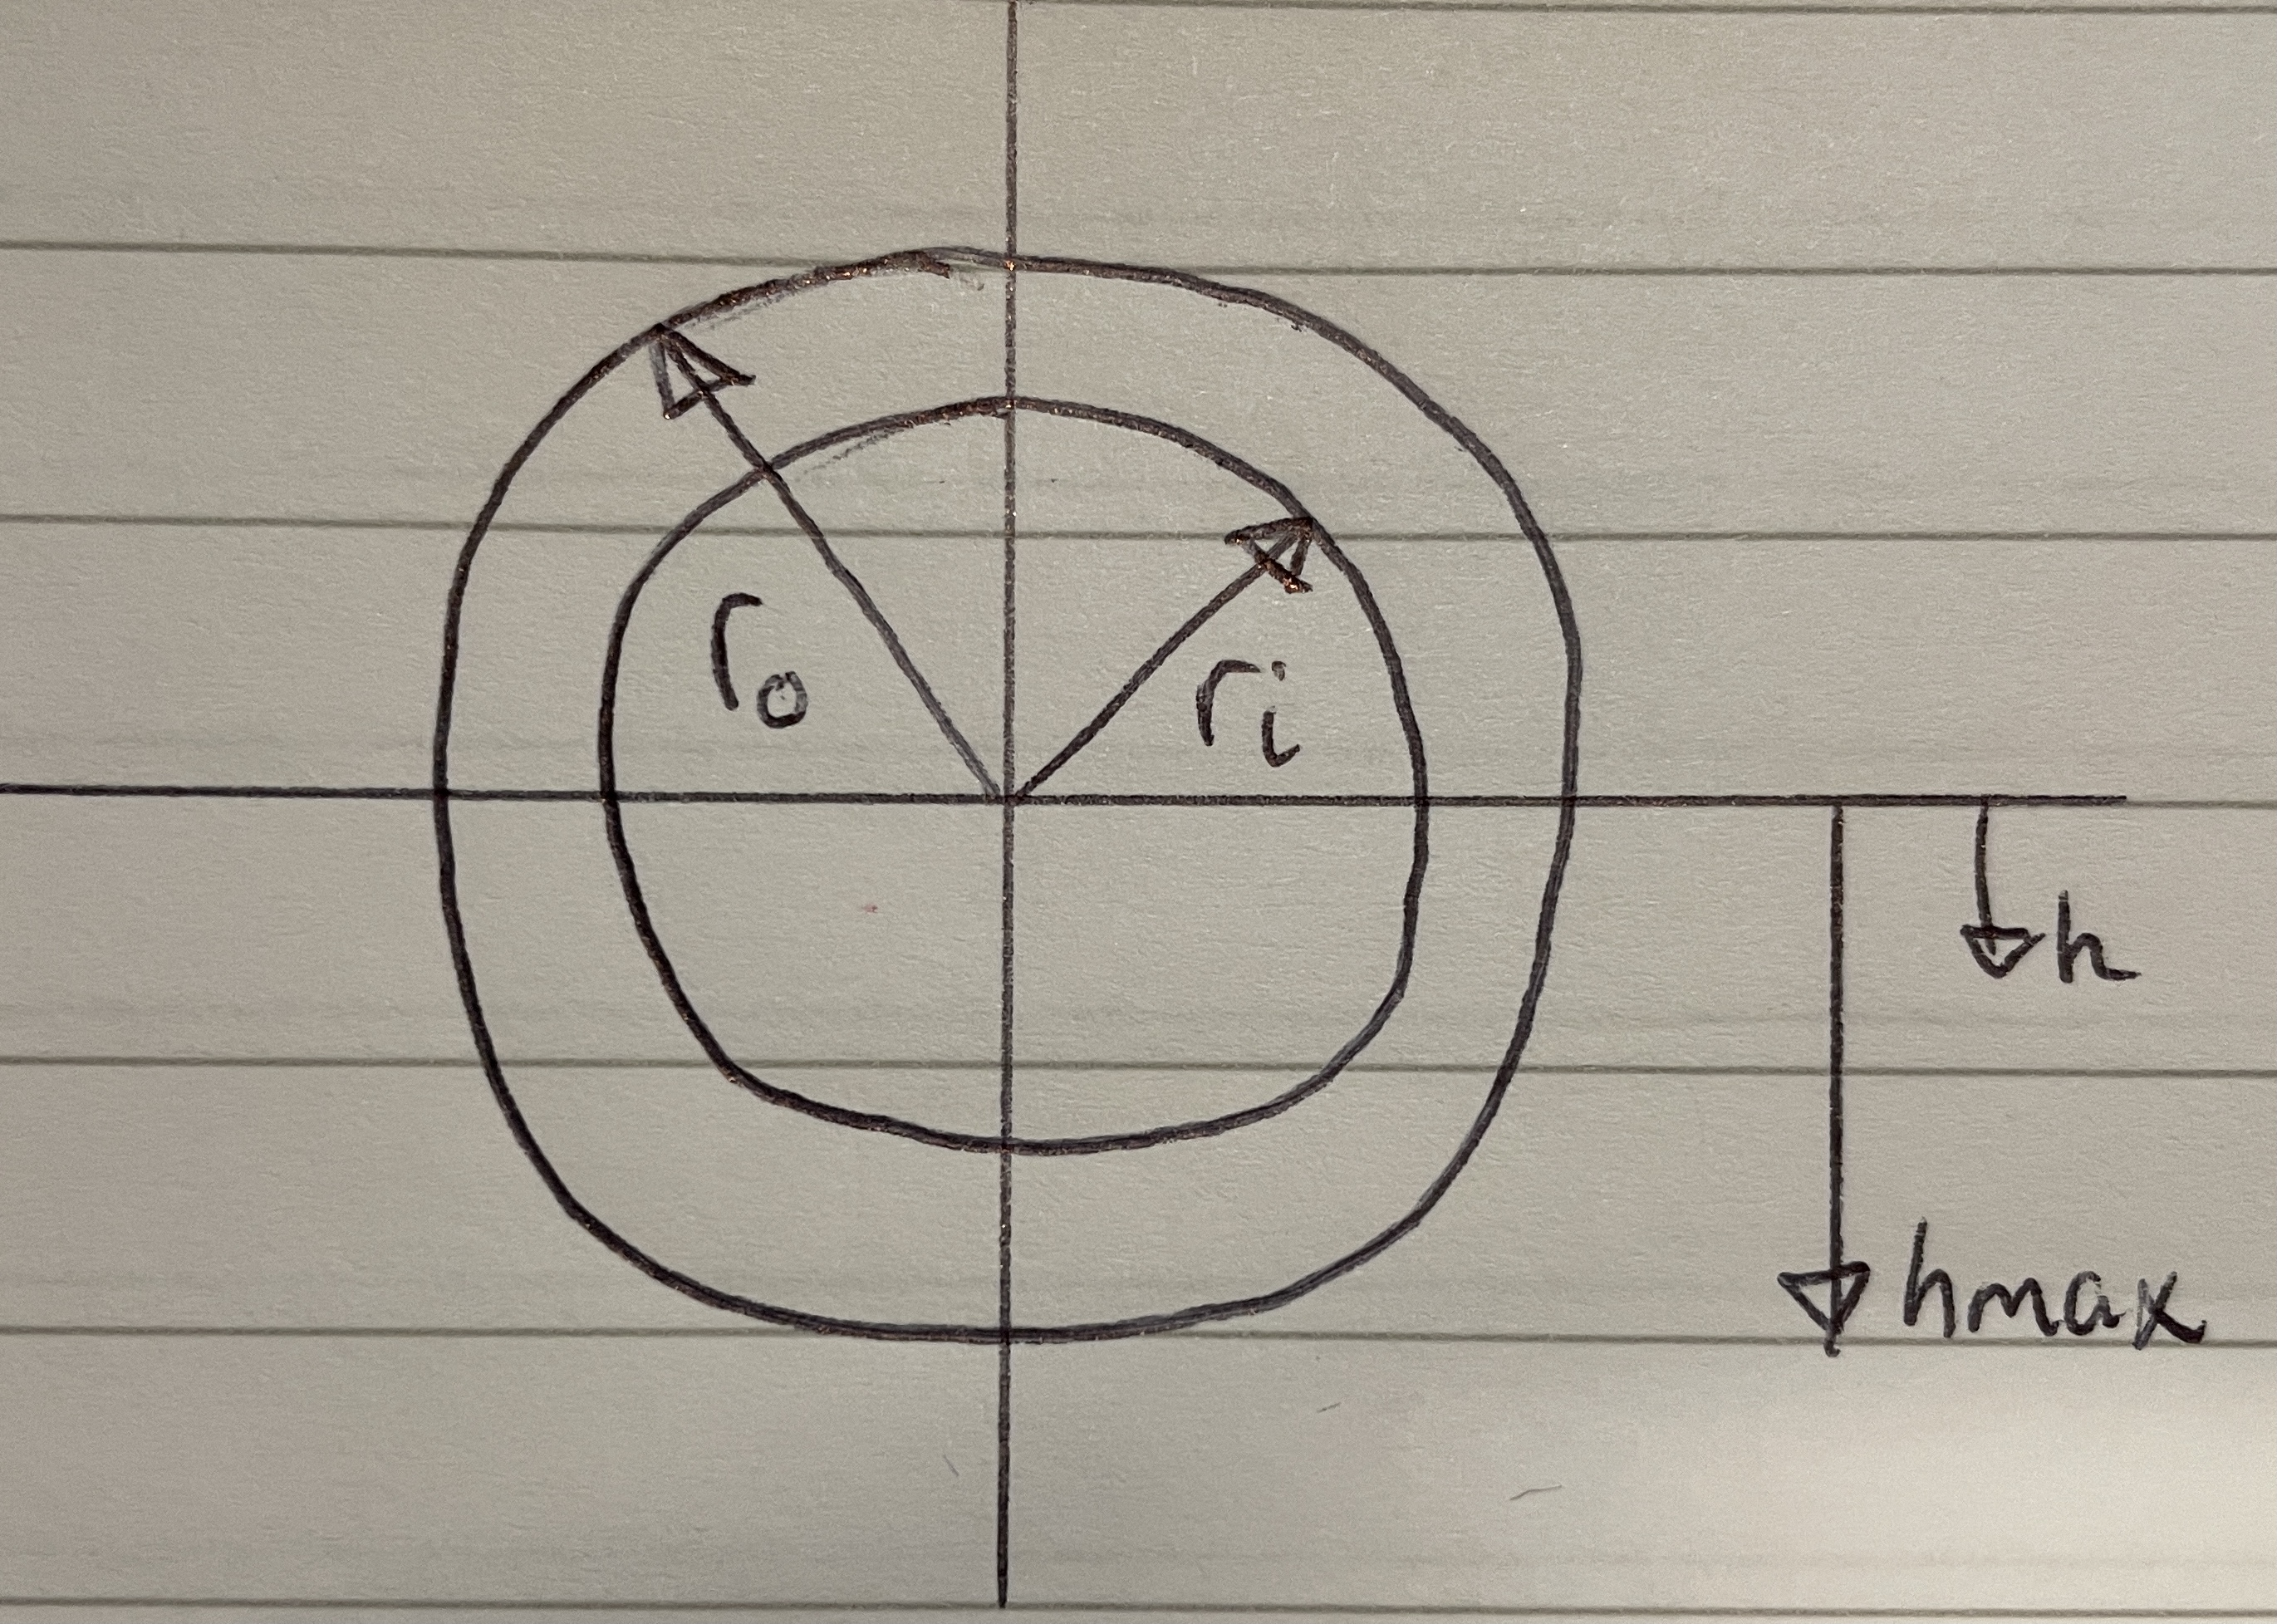
\includegraphics[height =5cm]{./img/q1iii.jpg}
    \caption{Diagram to show cross-section of horizontal beam.}
\end{figure}
Where $r_i = \SI{8.5}{\milli \meter}$, $r_o = \SI{10}{\milli \meter}$. The yield moment can be found using \ref{eq:q1iii1}:
\begin{equation}
    M_Y = \frac{\sigma_Y I}{h_{max}} \label{eq:q1iii1}
\end{equation}
Where $I = \frac{\pi}{4}\left(r_o^4-r_i^4\right)$ and $h_{max} = r_o$. Substituting:
\begin{align}
    M_Y &= \frac{480\times 10^6 \times \frac{\pi}{4}\left(0.01^4-0.0085^4\right)}{0.01}\\
    M_Y &= \SI{180.199}{\newton \meter} = \SI{180}{\newton \meter} \textrm{ (3sf)}
\end{align}
We now want to plot the bending moment as a function of $x$. MATLAB was used to plot Figure \ref{fig:q1iii}.
\lstset{language=Matlab,%
    %basicstyle=\color{red},
    breaklines=true,%
    morekeywords={matlab2tikz},
    keywordstyle=\color{blue},%
    morekeywords=[2]{1}, keywordstyle=[2]{\color{black}},
    identifierstyle=\color{black},%
    stringstyle=\color{mylilas},
    commentstyle=\color{mygreen},%
    showstringspaces=false,%without this there will be a symbol in the places where there is a space
    numbers=left,%
    numberstyle={\tiny \color{black}},% size of the numbers
    numbersep=9pt, % this defines how far the numbers are from the text
    emph=[1]{for,end,break},emphstyle=[1]\color{red}, %some words to emphasise
    %emph=[2]{word1,word2}, emphstyle=[2]{style},    
}
\lstinputlisting{./mCode/q1iii.m}
\begin{figure}[H]
    \centering
    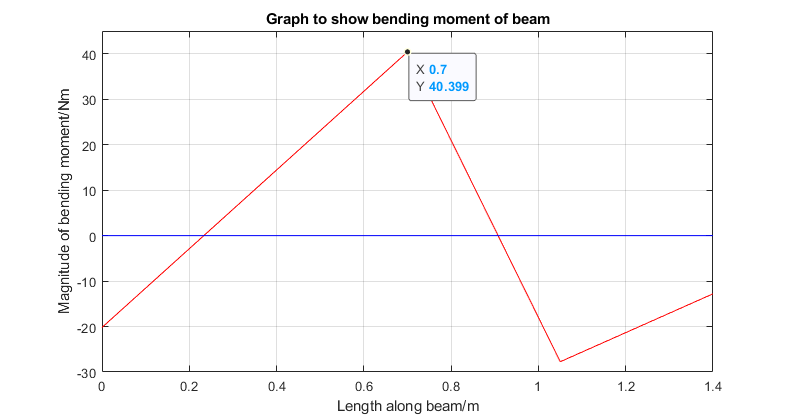
\includegraphics[width = \textwidth]{./img/q1iii2.png}
    \caption{Graph to show bending moment along the horizontal beam.}
    \label{fig:q1iii}
\end{figure}
We can see that from Figure \ref{fig:q1ii1} that the maximum bending moment at $x =2L$ is much lower than the yielding moment ($40.398<180$). We now want to find the $P$ value for which yielding will occur (at $2L$):
\begin{equation}
    M(x = 2L) = M_A + 2R_{Ay}L
\end{equation}
Substituting in $M_A$ and $R_{Ay}$ (\ref{q1iMA} and \ref{q1iRAy}):
\begin{align}
    M_A &= -\frac{2}{3}R_{Ay}L\\
    R_{Ay} &= \frac{3}{4}\left(P - \frac{WR}{L}-2W\right)\\
    M_A &= -\frac{2}{3}\left(\frac{3}{4}\left(P - \frac{WR}{L}-2W\right)\right)L\\
    M_A &= -\frac{L}{2} \left(P - \frac{WR}{L}-2W\right)\\
    M(x=2L) &= -\frac{1}{2}PL + \frac{1}{2}WR + WL + \frac{3}{2}PL - \frac{3}{2}WR - 3WL\\
    M &= PL - WR - 2WL
\end{align}
Let $M = M_Y$ and $P = P_Y$:
\begin{align}
    M_Y &= P_Y L - WR - 2WL\\
    P_Y &= \frac{1}{L}\left(M_Y + WR + 2WL\right)
\end{align}
Substituting the values of $M_Y$, $W$, $R$, $L$:
\begin{align}
    P_Y &= \frac{1}{0.35}\left(180.199+ 42.67\times 0.3 + 2\times 42.67 \times 0.35\right)\\
    P_Y &= \SI{636.769}{\newton} = \SI{637}{\newton} \textrm{ (3sf)}
\end{align}
From \ref{eq:q1i2}:
\begin{align}
    P &= \SI{237}{\newton} \textrm{ (3sf)}
\end{align}
Let us compare $P$ and $P_Y$ to confirm that the corrective load $P$ will not result in yielding:
\begin{align}
    P &< P_Y\\
    \SI{237}{\newton} &< \SI{637}{\newton}
\end{align}
Therefore, the corrective load will not result in engineering failure and the beam is safe.
\subsection{iv}
\begin{figure}[H]
    \centering
    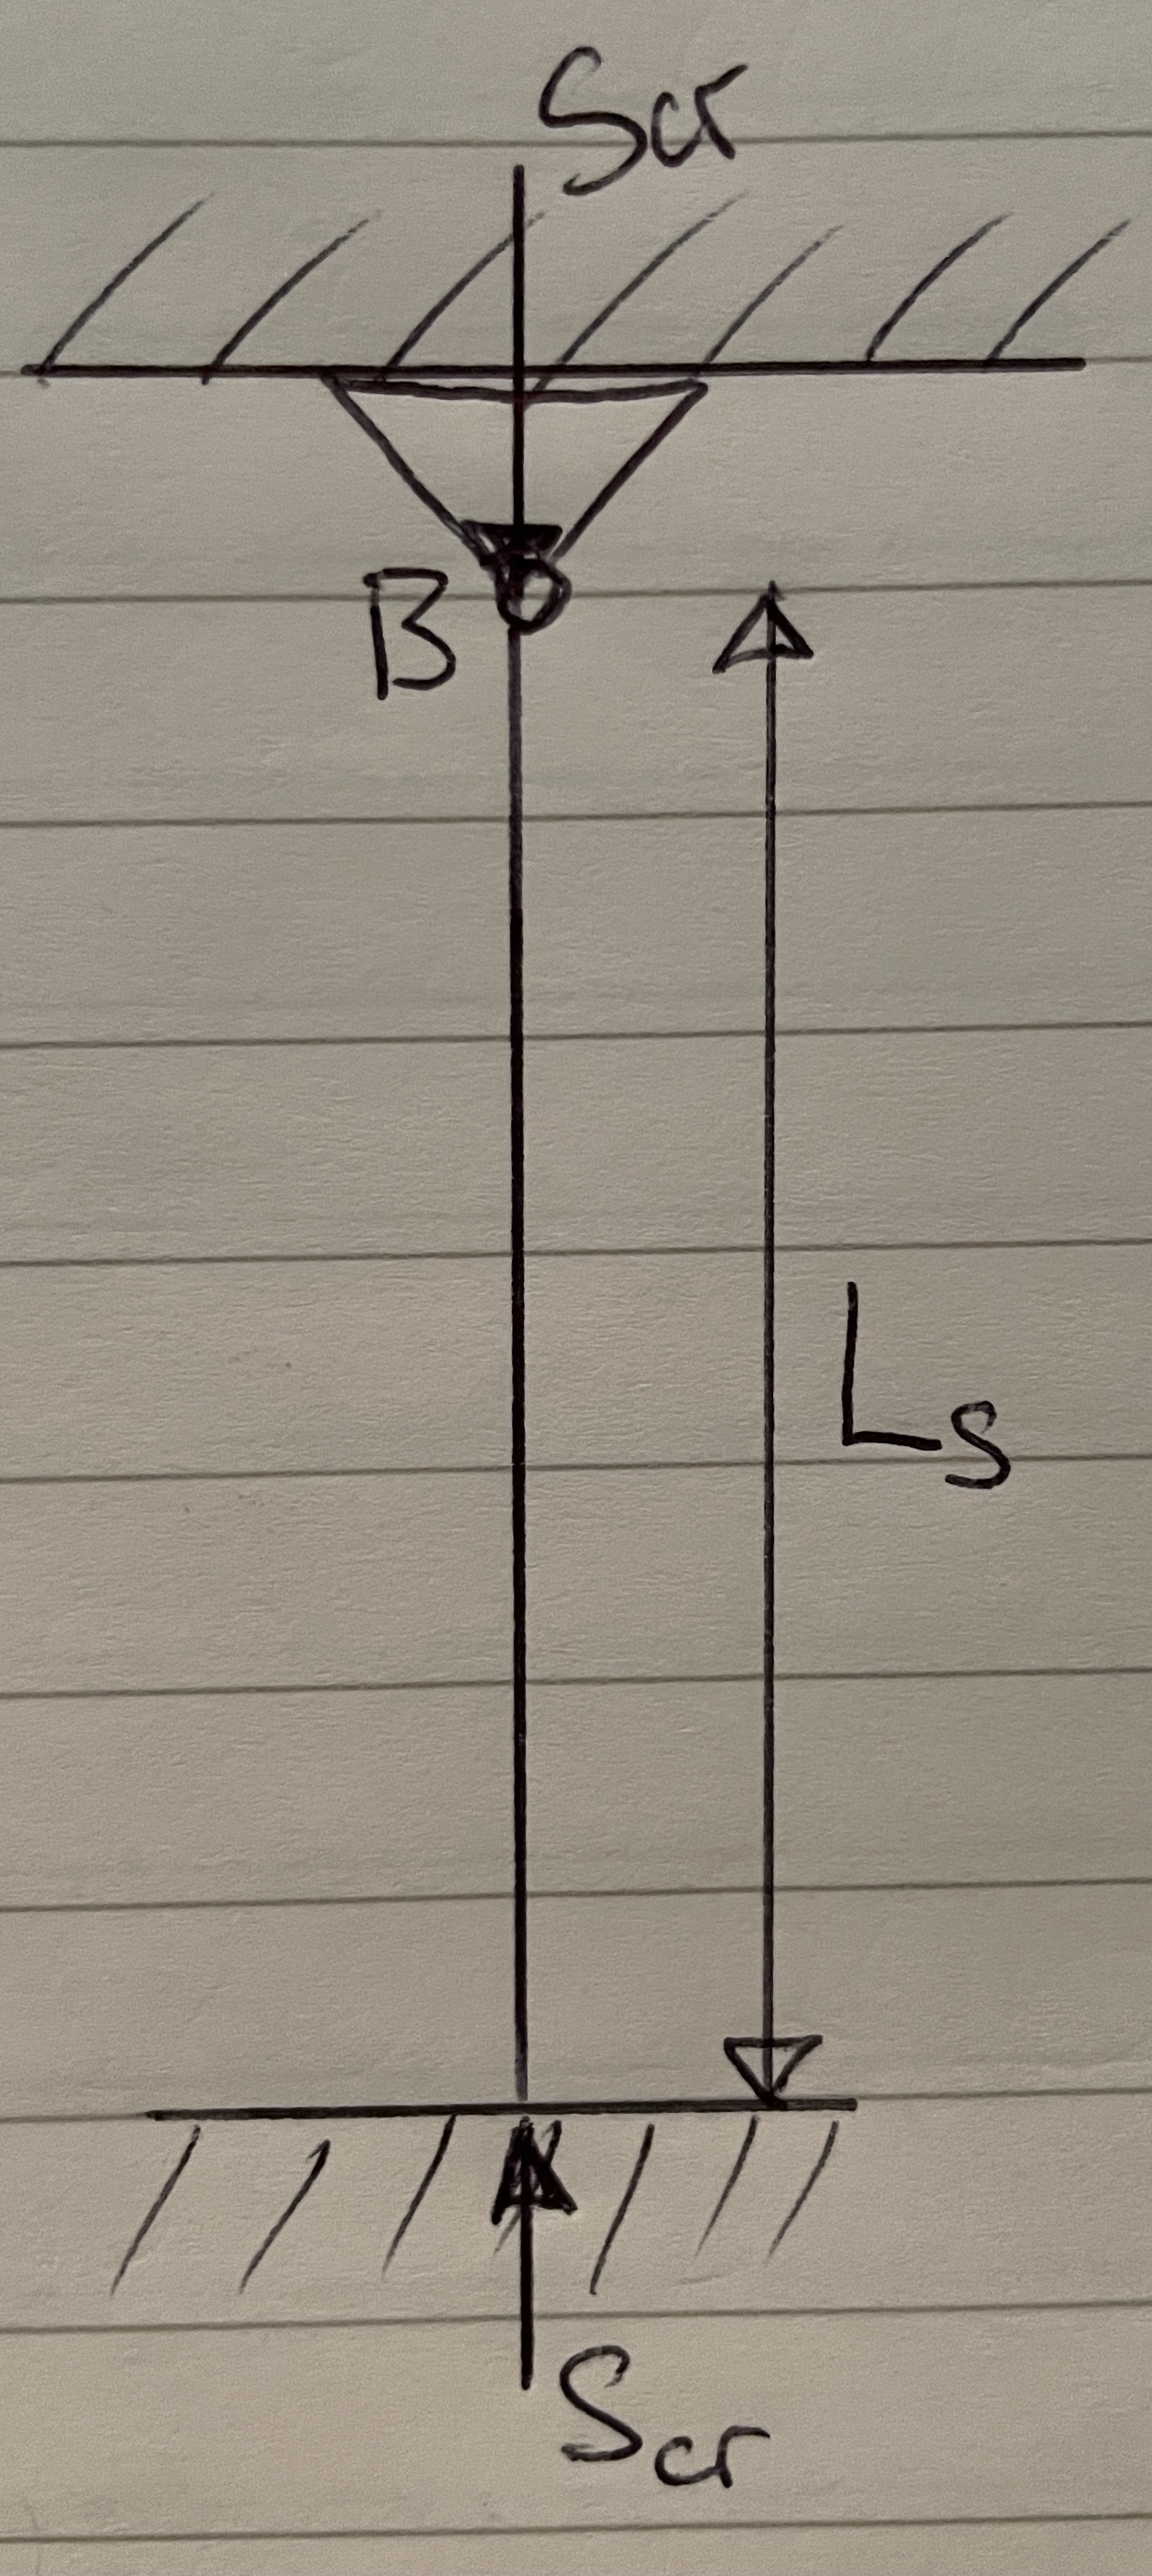
\includegraphics[height = 10cm]{./img/q1iv1.jpg}
    \caption{Graph to show arrangement of vertical strut at B.}
    \label{fig:q1iv}
\end{figure}
We can find the critical load using \ref{eq:q1iv1}:
\begin{equation}
    S_{cr} = \frac{n^2 \pi^2 EI}{L_e^2} \label{eq:q1iv1}
\end{equation}
Where $L_e = 0.7L_s$ for pinned-fixed columns. The second moment of inertia for the strut can be found using \ref{eq:q1iv2}:
\begin{equation}
    I = \frac{bh^3}{12} \label{eq:q1iv2}
\end{equation}
Where $b = 0.04$ and $h = 0.0045$. Calculating $I$ for each plane:
\begin{align}
    I_x &= \frac{bh^3}{12} = \frac{0.04\times 0.0045^3}{12} = \SI{3.0375e-10}{\meter\tothe{4}}\\
    I_y &= \frac{b^3h}{12} = \frac{0.04^3\times 0.0045}{12} = \SI{2.4e-8}{\meter\tothe{4}}
\end{align}
Buckling occurs in the plane with the lowest $I$, hence buckling will occur in the $x$-plane first. Testing:
\begin{align}
    S_{cr} &= \frac{1\times \pi^2 \times 71\times 10^{9}\times \frac{0.04\times 0.0045^3}{12}}{(0.7\times0.96)^2}\\
    S_{cr} &= \SI{471.342}{\newton} = \SI{471}{\newton} \textrm{ (3sf)}
\end{align}
For the value of $P$ which we calculated in part i, $R_B$ is pulling the strut in tension and hence is safe from buckling. We can compare the value of $R_B$ to our $S_{cr}$ value, when $P$ is 0; this value can be found by adjusting the MATLAB code to $P=0$ in part i and generating the output for $R_B$.
\begin{align}
    R_B &< S_{cr}\\
    \SI{134}{\newton} &< \SI{471}{\newton}
\end{align}
Critical load is not reached, hence the strut is suitable and will not fail under these conditions. 
\section{Question 2}
\subsection{i}
\begin{figure}[H]
    \centering
    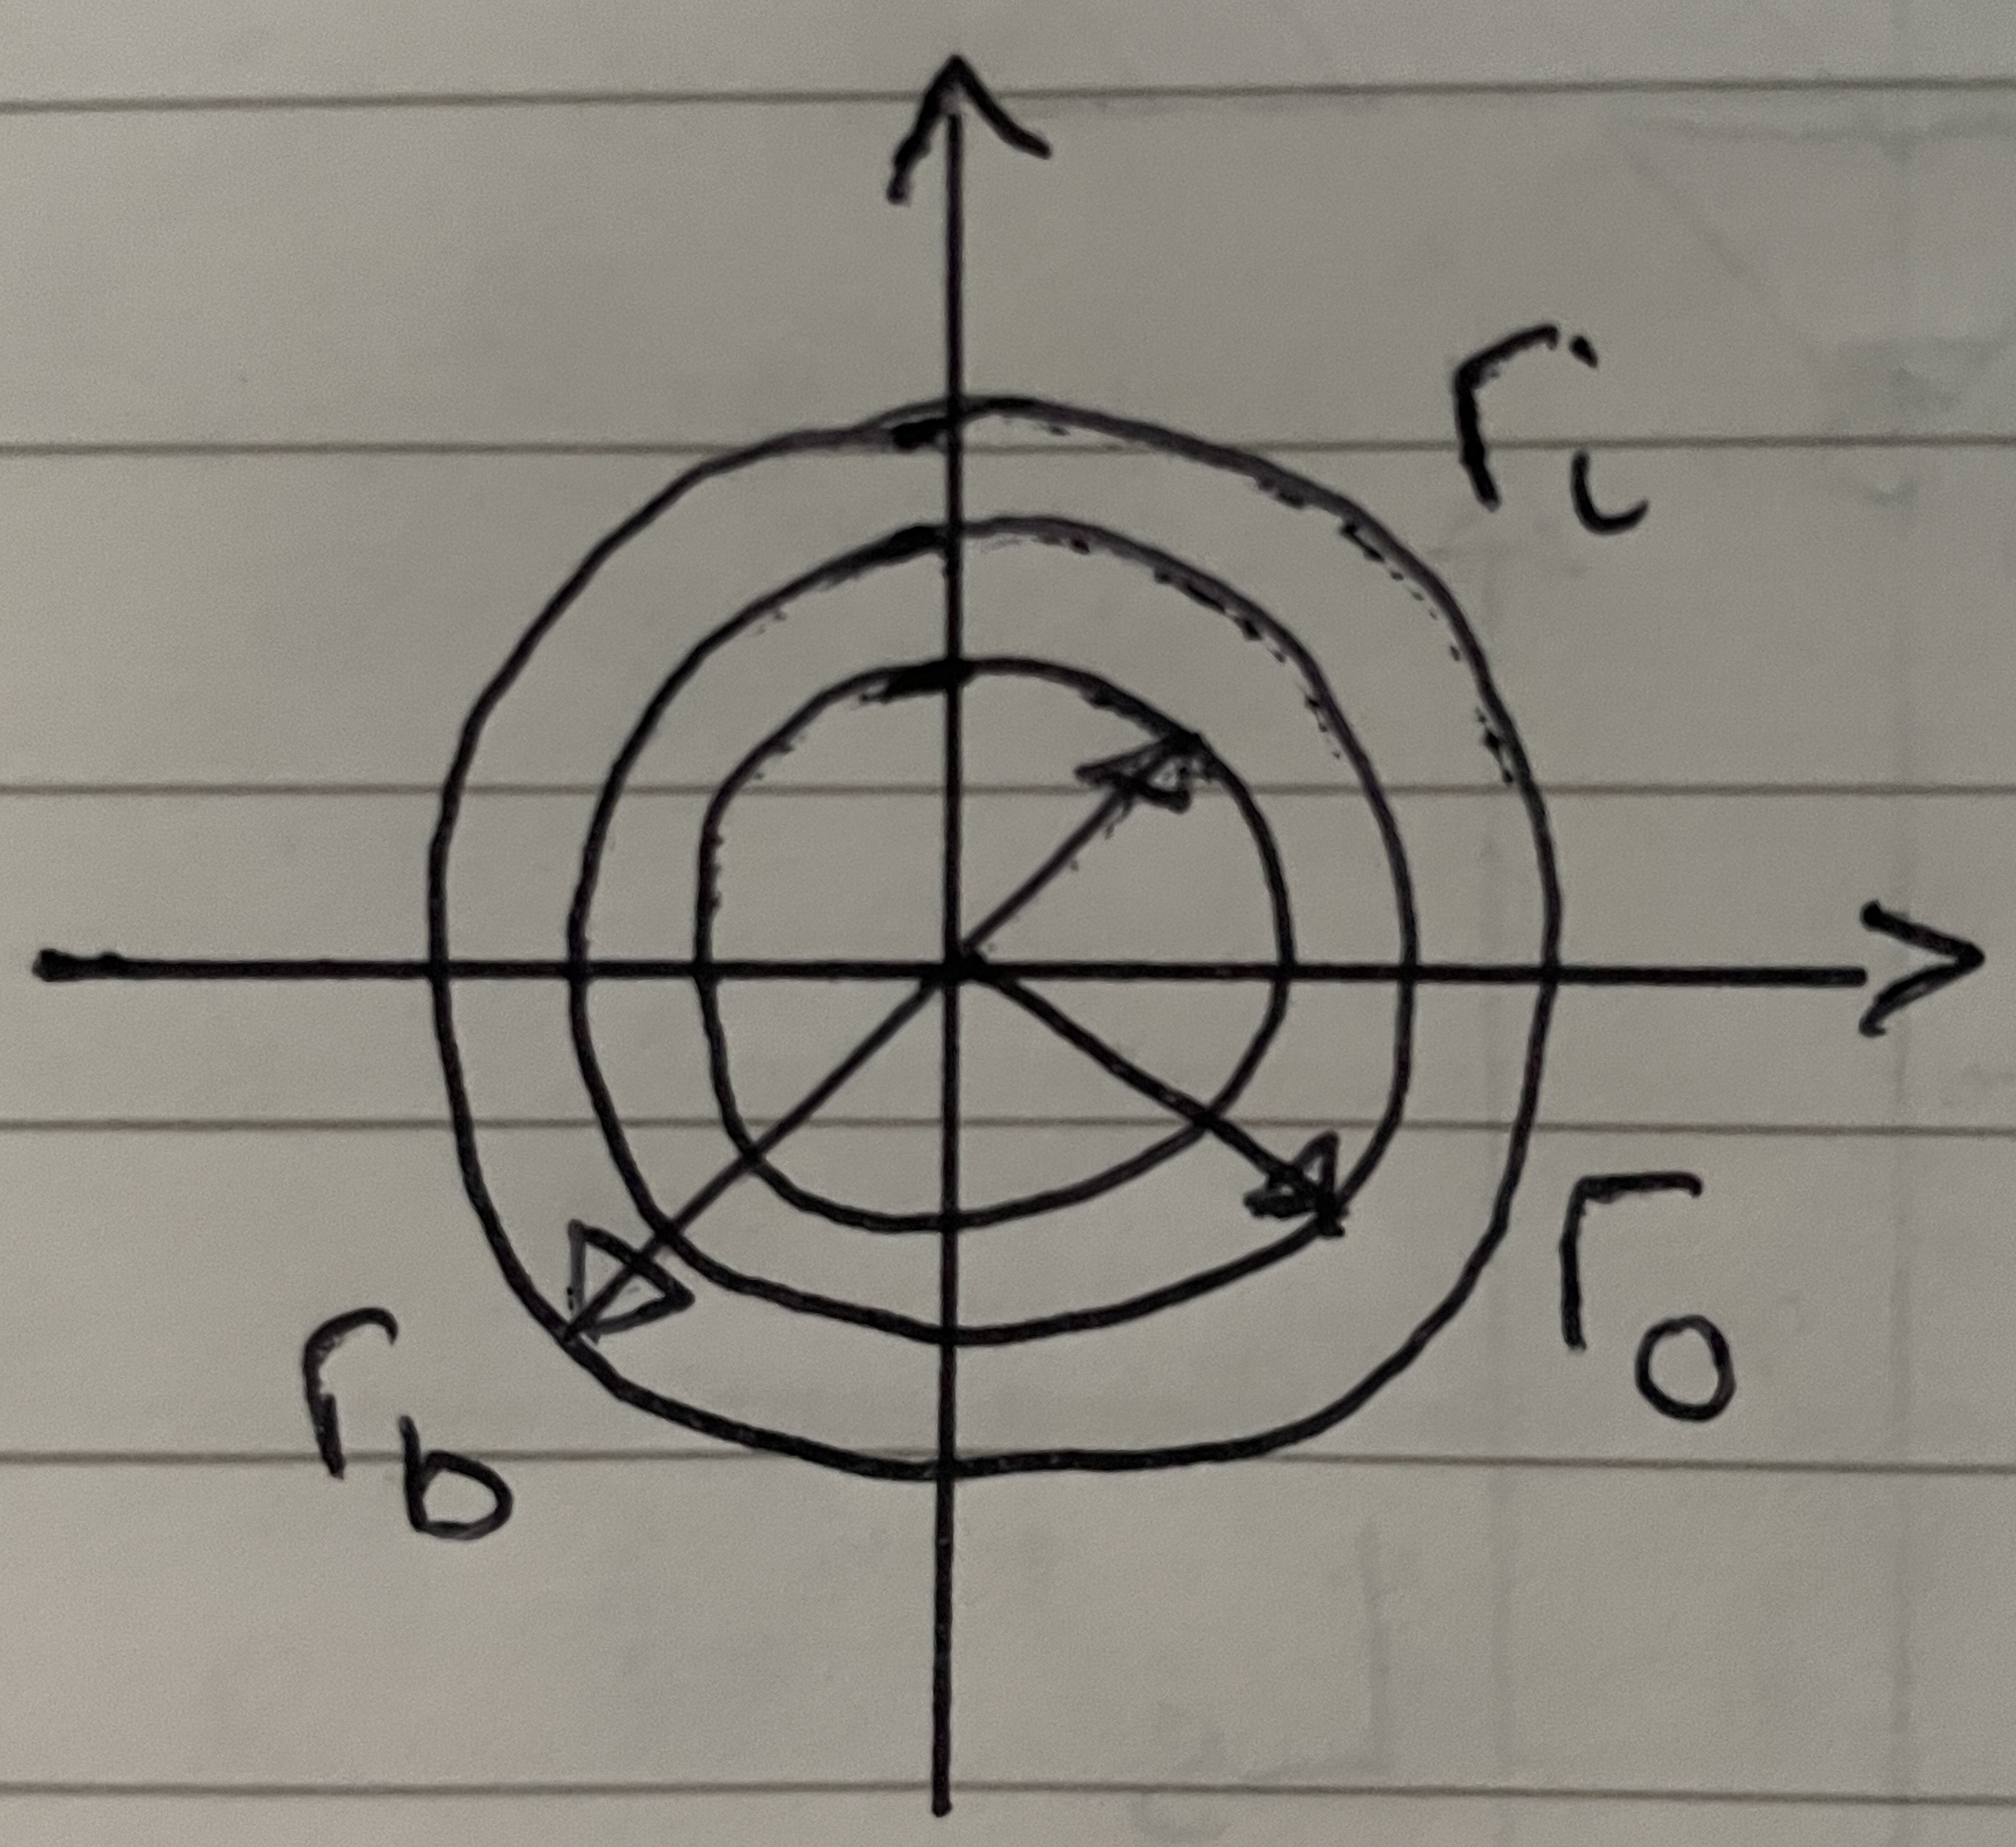
\includegraphics[height =5cm]{./img/q2i2.jpg}
    \caption{Sketch of cylinder arrangement.}
\end{figure}
\begin{figure}[H]
    \centering
    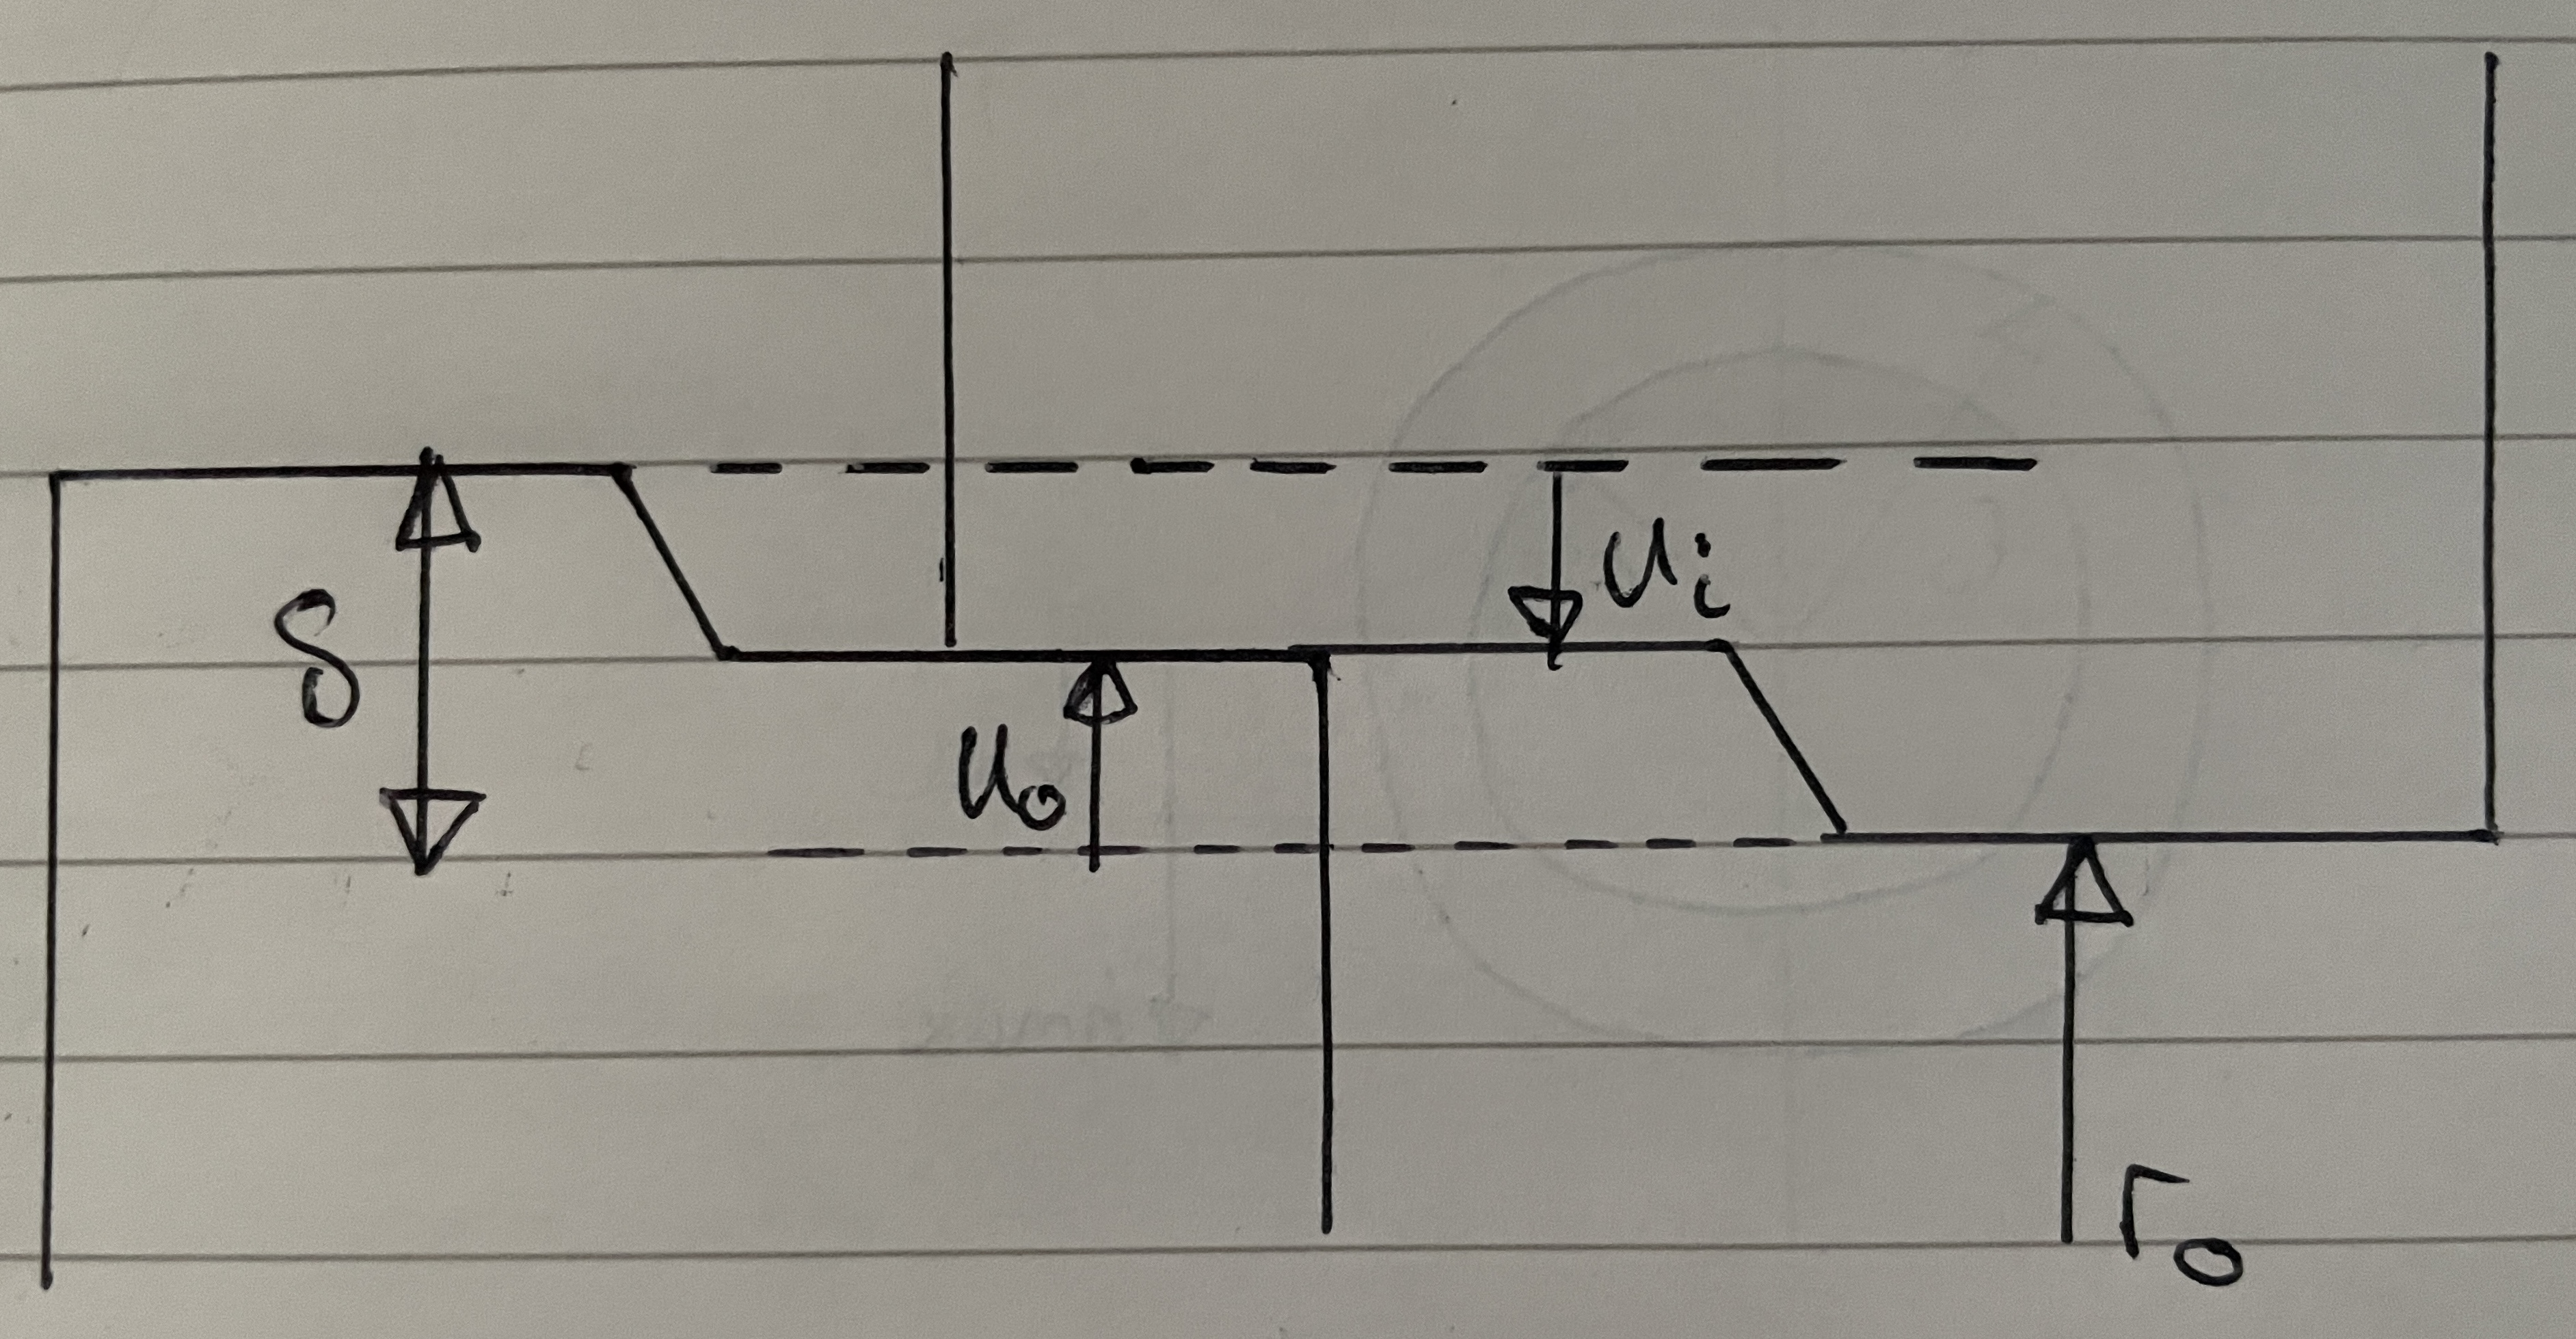
\includegraphics[height =5cm]{./img/q2i1.jpg}
    \caption{Diagram to show interference.}
\end{figure}
Hence:
\begin{equation}
    \delta = u_o - u_i
\end{equation}
Finding $u_i$. Let us start with the general equation for $u$:
\begin{gather}
    u = \frac{r}{E}\left(\sigma_{\theta} - v \sigma_r\right)\\
    \rightarrow u_i = \frac{r_o}{E_i}\left[\sigma_{\theta, i} \left(r_o\right) - v_i \sigma_{r,i} (r_o)\right]
\end{gather}
Lame's equations:
\begin{gather}
    \sigma_r = A - \frac{B}{r^2}\\
    \sigma_{\theta} = A + \frac{B}{r^2}
\end{gather}
Boundary conditions:
\begin{gather}
    \sigma_{r,i}(r_i) = 0 = A - \frac{B}{r_i^2}\\
    \sigma_{r,i}(r_o) = -p_{int} = A - \frac{B}{r_o^2}\\
    A = -p_{int}\frac{r_o^2}{r_o^2 - r_i^2}\\
    B = -p_{int}\frac{r_i^2 \cdot r_o^2}{r_o^2 - r_i^2}
\end{gather}
Substituting:
\begin{equation}
    \sigma_{\theta,i} = A + \frac{B}{r^2} = -p_{int}\frac{r_o^2}{r_o^2 - r_i^2} \left(1 + \frac{r_i^2}{r^2}\right) \label{eq:q2ii1}
\end{equation}
Therefore:
\begin{gather}
    \sigma_{r,i}(r_o) = -p_{int} \hspace{1cm} \sigma_{\theta,i}(r_o) = -p_{int}\frac{r_o^2 + r_i^2}{r_o^2 - r_i^2}\\
    u_i = -p_{int} \frac{r_o}{E_i} \left(\frac{r_o^2 + r_i^2}{r_o^2 - r_i^2} - v_i\right)
\end{gather}
Repeating to find $u_o$:
\begin{gather}
    u_o = \frac{r_o}{E_o}\left[\sigma_{\theta,o} (r_o) - v_o \sigma_{r,o}(r_o)\right]
\end{gather}
Lame's equations:
\begin{gather}
    \sigma_r = A - \frac{B}{r^2}\\
    \sigma_{\theta} = A + \frac{B}{r^2}
\end{gather}
Boundary conditions:
\begin{gather}
    \sigma_{r,o}(r_o) = p_{int} = A - \frac{B}{r_o^2}\\
    \sigma_{r,o}(r_b) = 0 = A - \frac{B}{r_b^2}\\
    A = p_{int} \frac{r_o^2}{r_o^2- r_b^2}\\
    B = p_{int} \frac{r_o^2 \cdot r_b^2}{r_b^2 - r_o^2}
\end{gather}
Substituting:
\begin{gather}
    \sigma_{\theta,o} = A + \frac{B}{r^2} = p_{int} \frac{r_o^2}{r_b^2 - r_o^2} \left(1+ \frac{r_b^2}{r^2}\right) \label{eq:q2ii2}
\end{gather}
Therefore:
\begin{gather}
    \sigma_{r,o}(r_b) = 0 \hspace{1cm} \sigma_{\theta,o}(r_o) = p_{int}\frac{r_b^2 + r_o^2}{r_b^2 -r_o^2}\\
    u_o = p_{int} \frac{r_o}{E_o}\left(\frac{r_b^2 + r_o^2}{r_b^2 - r_o^2} + v_o\right)
\end{gather}
Finding $\delta$:
\begin{gather}
    u_i =-p_{int}\frac{r_o}{E_i}\left(\frac{r_o^2 + r_i^2 }{r_o^2 - r_i^2}-v_i\right)\\
    u_o = p_{int}\frac{r_o}{E_o}\left(\frac{r_b^2 + r_o^2 }{r_b^2 - r_o^2}+v_o\right)\\
    \delta = p_{int}r_o\left[\frac{1}{E_o}\left(\frac{r_b^2 + r_o^2}{r_b^2 - r_o^2}+v_o\right) + \frac{1}{E_i}\left(\frac{r_o^2 + r_i^2}{r_o^2 - r_i^2}-v_i\right)\right]
\end{gather}
For a single material: $E_i = E_o = E$, and $v_i = v_o = v$:
\begin{gather}
    \delta = p_{int} \frac{r_o}{E}\left[\frac{2r_o^2\left(r_b^2-r_i^2\right)}{\left(r_b^2 - r_o^2\right)\left(r_o^2-r_i^2\right)}\right] \\
    p_{int} = E \delta \left[\frac{\left(r_b^2 - r_o^2\right)\left(r_o^2 - r_b^2\right)}{2r_o^3\left(r_b^2 - r_i^2\right)}\right]
\end{gather}
Converting radius to diameters:
\begin{gather}
    \delta = p_{int} \frac{d_o}{E}\left[\frac{d_o^2\left(d_b^2-d_i^2\right)}{\left(d_b^2 - d_o^2\right)\left(d_o^2-d_i^2\right)}\right] \label{q2idelta}\\
    p_{int} = E \delta \left[\frac{\left(d_b^2 - d_o^2\right)\left(d_o^2 - d_b^2\right)}{d_o^3\left(d_b^2 - d_i^2\right)}\right]
\end{gather}
Where $\delta$ is the radial interference.
\subsection{ii}
We can find the internal pressure through the following equation:
\begin{align}
    F &\leq PA\mu_s
    F &\leq \pi d_o L_b p_{int} \mu_s\\
    p_{int} &\geq \frac{F}{\pi d_o L_b \mu_s}\\
    p_{int} &\geq \frac{10000}{\pi (20\times 10^{-3})(50\times 10^{-3})(0.8)}\\
    p_{int} &\geq \SI{3978873.577}{\pascal}
\end{align}
Using a value of \SI{4e6}{\pascal} for $p_{int}$, we can now substitute into \ref{q2idelta}:
\begin{align}
    \delta &= \frac{(4\times 10^{6})(20\times 10^{-3})}{210\times 10^9}\left[\frac{(20\times 10^{-3})^2\left((23\times 10^{-3})^2-(17\times 10^{-3})^2\right)}{\left((23\times 10^{-3})^2 - (20\times 10^{-3})^2\right)\left((20\times 10^{-3})^2-(17\times 10^{-3})^2\right)}\right]\\
    \delta &= \SI{2.554e-6}{\meter} = \SI{0.00255}{\milli\meter}
\end{align}
Where $\delta$ is the radial interference. We need to make sure that this interference value does not result in the engineering failure of the internal or external cylinder. Looking at the internal cylinder, we can find the stress by utilising Lame's equations (\ref{eq:q2ii1} and \ref{eq:q2ii2}):
\begin{align}
    \sigma_{ri} \left(r_o\right) &= -p_{int} = \SI{-4e6}{\pascal}\\
    \sigma_{\theta i} \left(r_o\right) &= -p_{int}\frac{r_o^2 + r_i^2}{r_o^2 - r_i^2} = -4\times 10^6 \cdot \frac{0.01^2 + 0.0085^2}{0.01^2 - 0.0085^2} = \SI{-2.483e7}{\pascal}\\
    \sigma_{ro} \left(r_o\right) &= p_{int} = \SI{4e6}{\pascal}\\
    \sigma_{\theta o} \left(r_o\right) &= p_{int}\frac{r_b^2 + r_o^2}{r_b^2 -r_o^2} = 4\times 10^6 \cdot \frac{0.0115^2 + 0.01^2}{0.0115^2 -0.01^2} = \SI{2.881e7}{\pascal}
\end{align}
We can use the distortion-energy theory to calculate the strain energy in the tubes. This theory is justified as it is the most reliable method for calculating the stress. The strain energy associated with distortion can be found using \ref{eq:q2ii3} and this must be lower than the yield stress $\sigma_Y$:
\begin{align}
    \sigma_i &< \sigma_Y\\
    \sqrt{\frac{\sigma_{ri}^2 + \sigma_{\theta i}^2 + \left(\sigma_{ri} - \sigma_{\theta i}\right)^2}{2}} &< \sigma_Y \label{eq:q2ii3}\\
    \sqrt{\frac{(-4\times10^6)^2 + (-2.483\times 10^7)^2 + \left((-4\times 10^6) - (-2.483\times 10^7)\right)^2}{2}} &< 4.8\times 10^8\\
    2.309\times 10^7 &< 4.8 \times 10^8
\end{align}
Hence, inner tube is not subject to yielding stress. Repeating for outer tube:
\begin{align}
    \sigma_o &< \sigma_Y\\
    \sqrt{\frac{\sigma_{ro}^2 + \sigma_{\theta o}^2 + \left(\sigma_{ro} - \sigma_{\theta o}\right)^2}{2}} &< \sigma_Y\\
    \sqrt{\frac{(4\times10^6)^2 + (2.881\times 10^7)^2 + \left((4\times 10^6) - (2.881\times 10^7)\right)^2}{2}} &< 4.8\times 10^8\\
    2.703\times 10^7 &< 4.8 \times 10^8
\end{align}
Hence, outer tube is not subject to yielding stress.
\subsection{iii}
Equations to form the Mohr's circle were put into MATLAB and circles formed and plotted. Calculations for key values were also made and are listed below.
\lstset{language=Matlab,%
    %basicstyle=\color{red},
    breaklines=true,%
    morekeywords={matlab2tikz},
    keywordstyle=\color{blue},%
    morekeywords=[2]{1}, keywordstyle=[2]{\color{black}},
    identifierstyle=\color{black},%
    stringstyle=\color{mylilas},
    commentstyle=\color{mygreen},%
    showstringspaces=false,%without this there will be a symbol in the places where there is a space
    numbers=left,%
    numberstyle={\tiny \color{black}},% size of the numbers
    numbersep=9pt, % this defines how far the numbers are from the text
    emph=[1]{for,end,break},emphstyle=[1]\color{red}, %some words to emphasise
    %emph=[2]{word1,word2}, emphstyle=[2]{style},    
}
\lstinputlisting{./mCode/q2iii.m}
\begin{figure}[H]
    \centering
    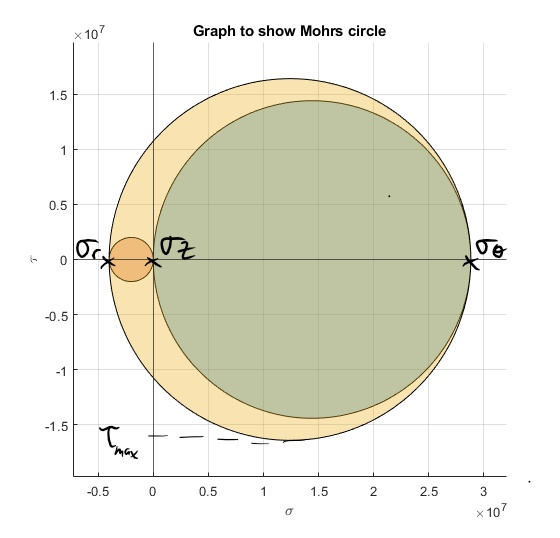
\includegraphics[height = 10cm]{./img/Inkedq2iii1_LI.jpg}
    \caption{Graph to show Mohr's circle.}
    \label{fig:q2iii}
\end{figure}
Where the value of $\sigma_r = \SI{-4e6}{\pascal}$, $\sigma_z = \SI{0}{\pascal}$, $\sigma_{\theta} = \SI{2.88e7}{\pascal}$ and $\tau_{max} = \SI{1.64e7}{\pascal}$
\section{Question 3}
\subsection{i}
\begin{figure}[H]
    \centering
    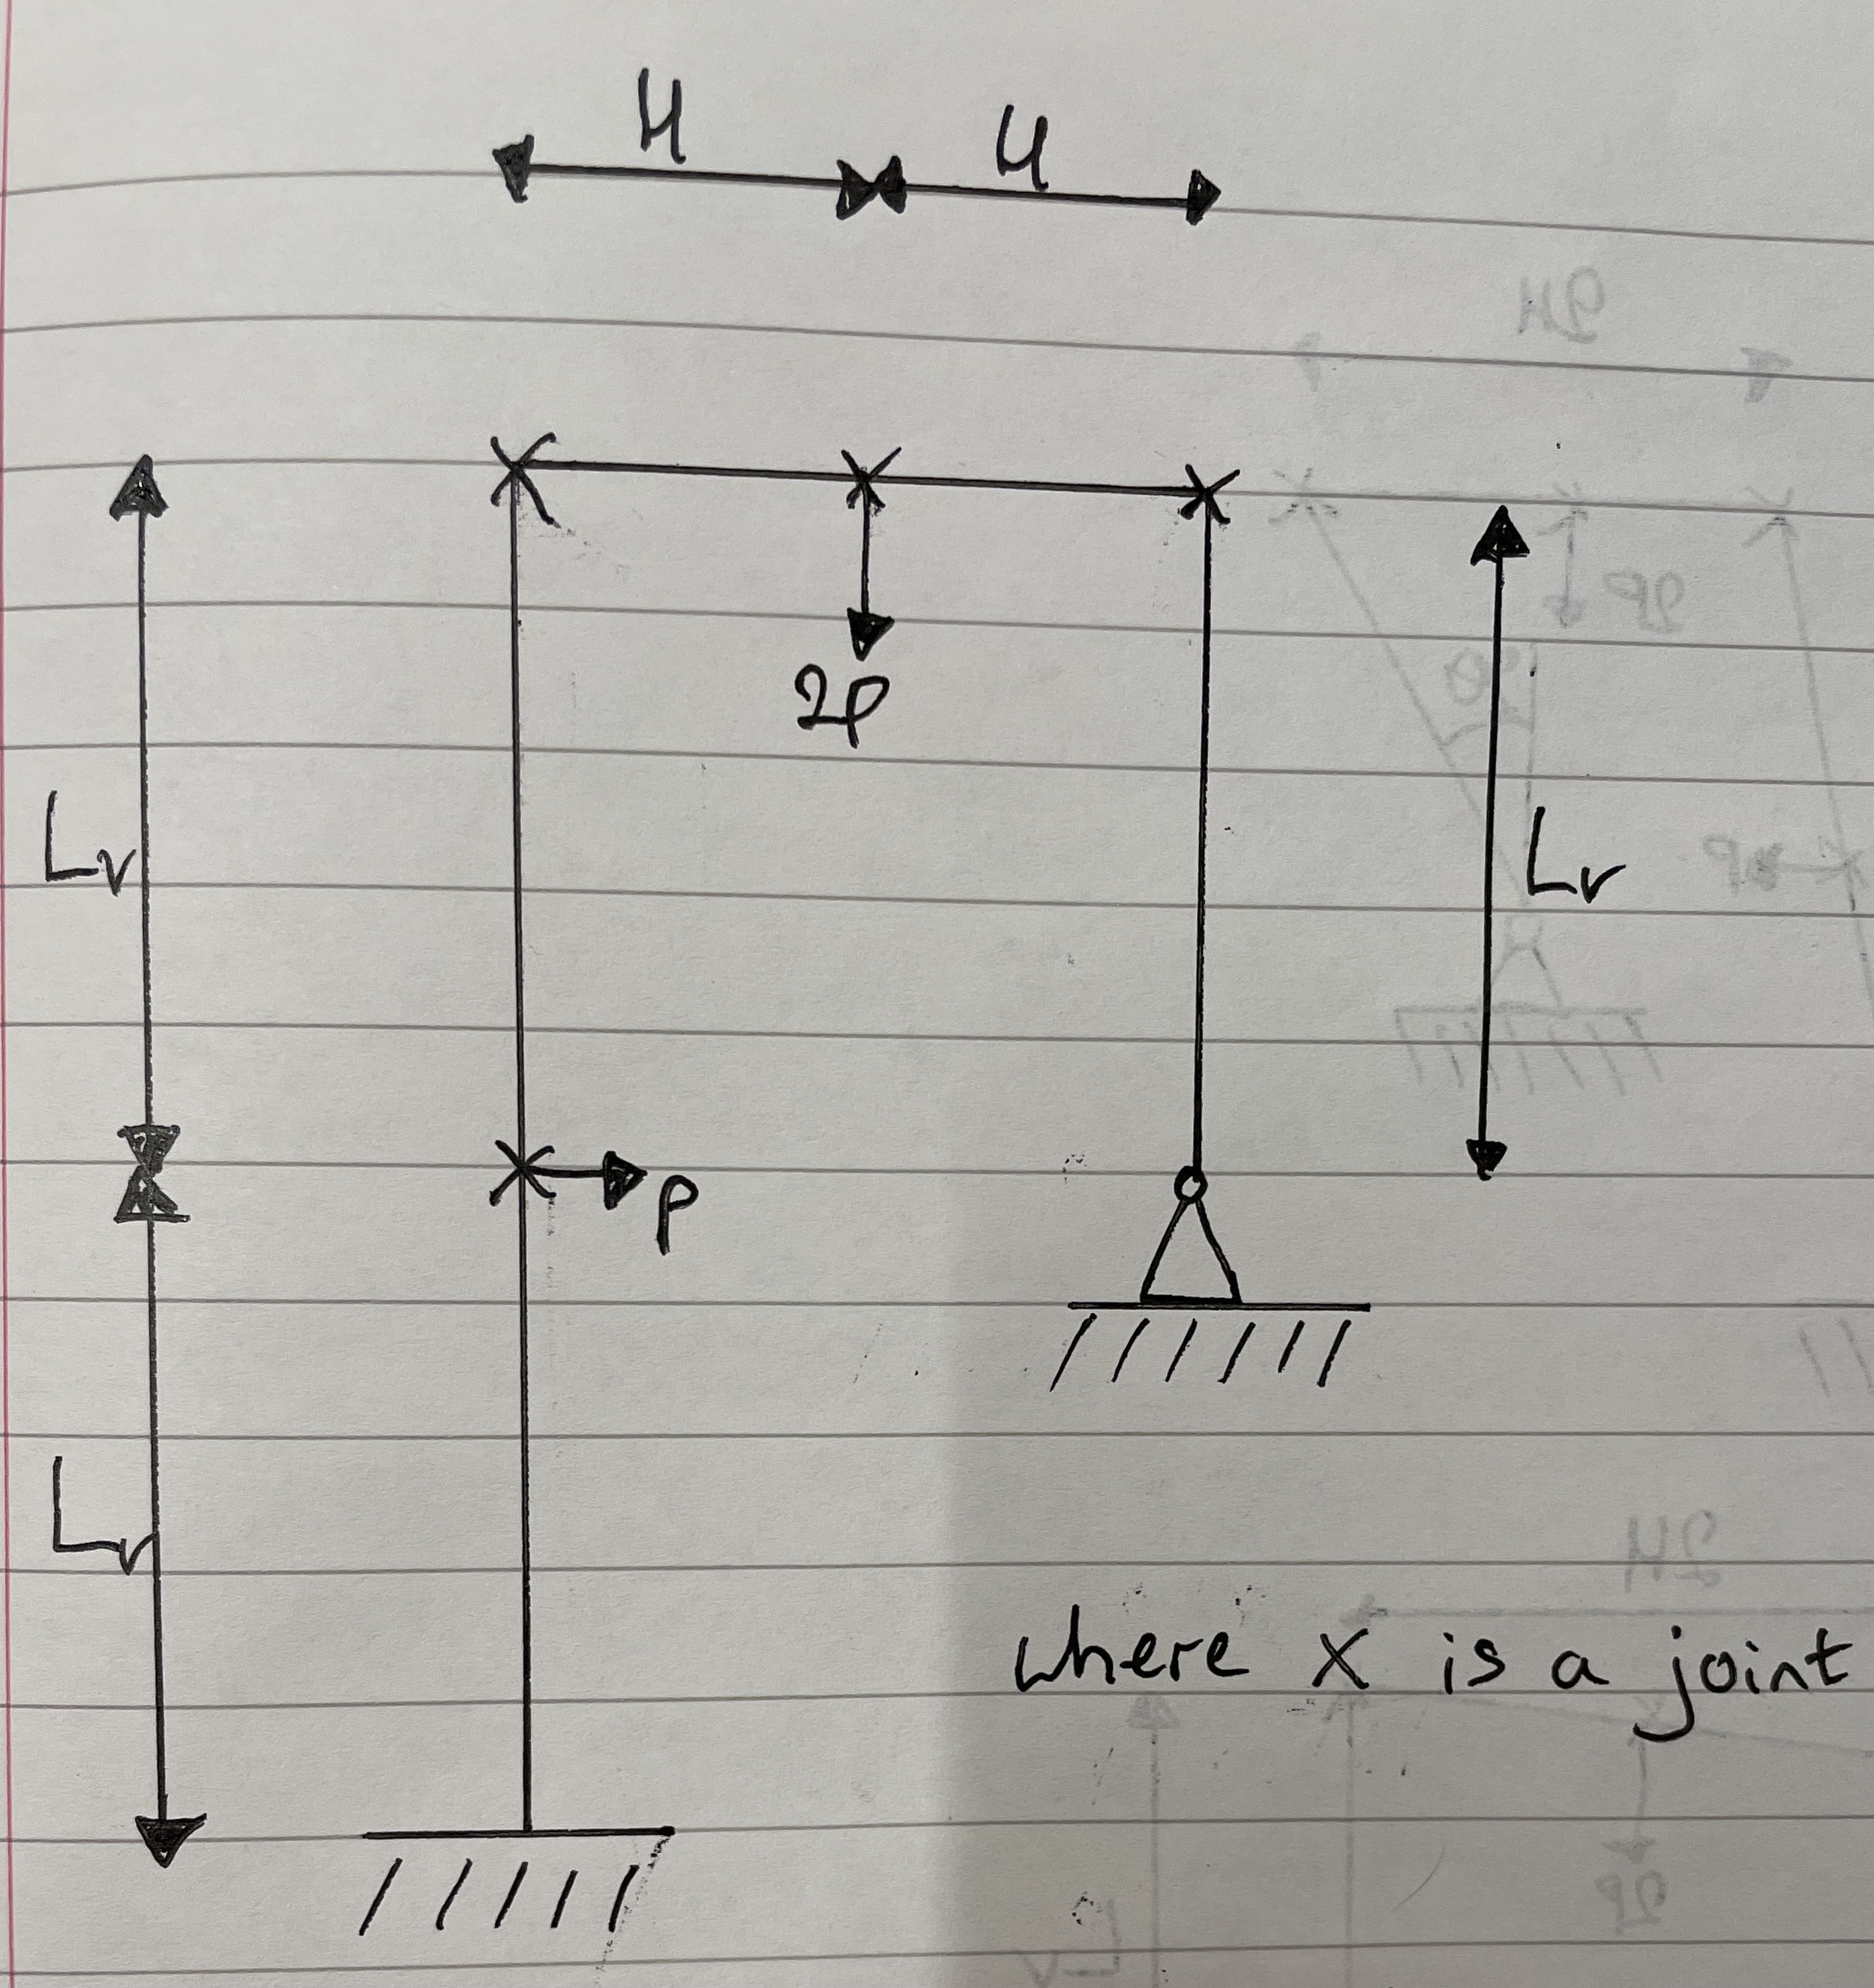
\includegraphics[width = 0.9\textwidth]{./img/q3i1.jpg}
    \caption{Sketch of portal frame.}
\end{figure}
\newpage
We can now look at the potential modes of collapse of the portal frame. 
\begin{figure}[H]
    \centering
    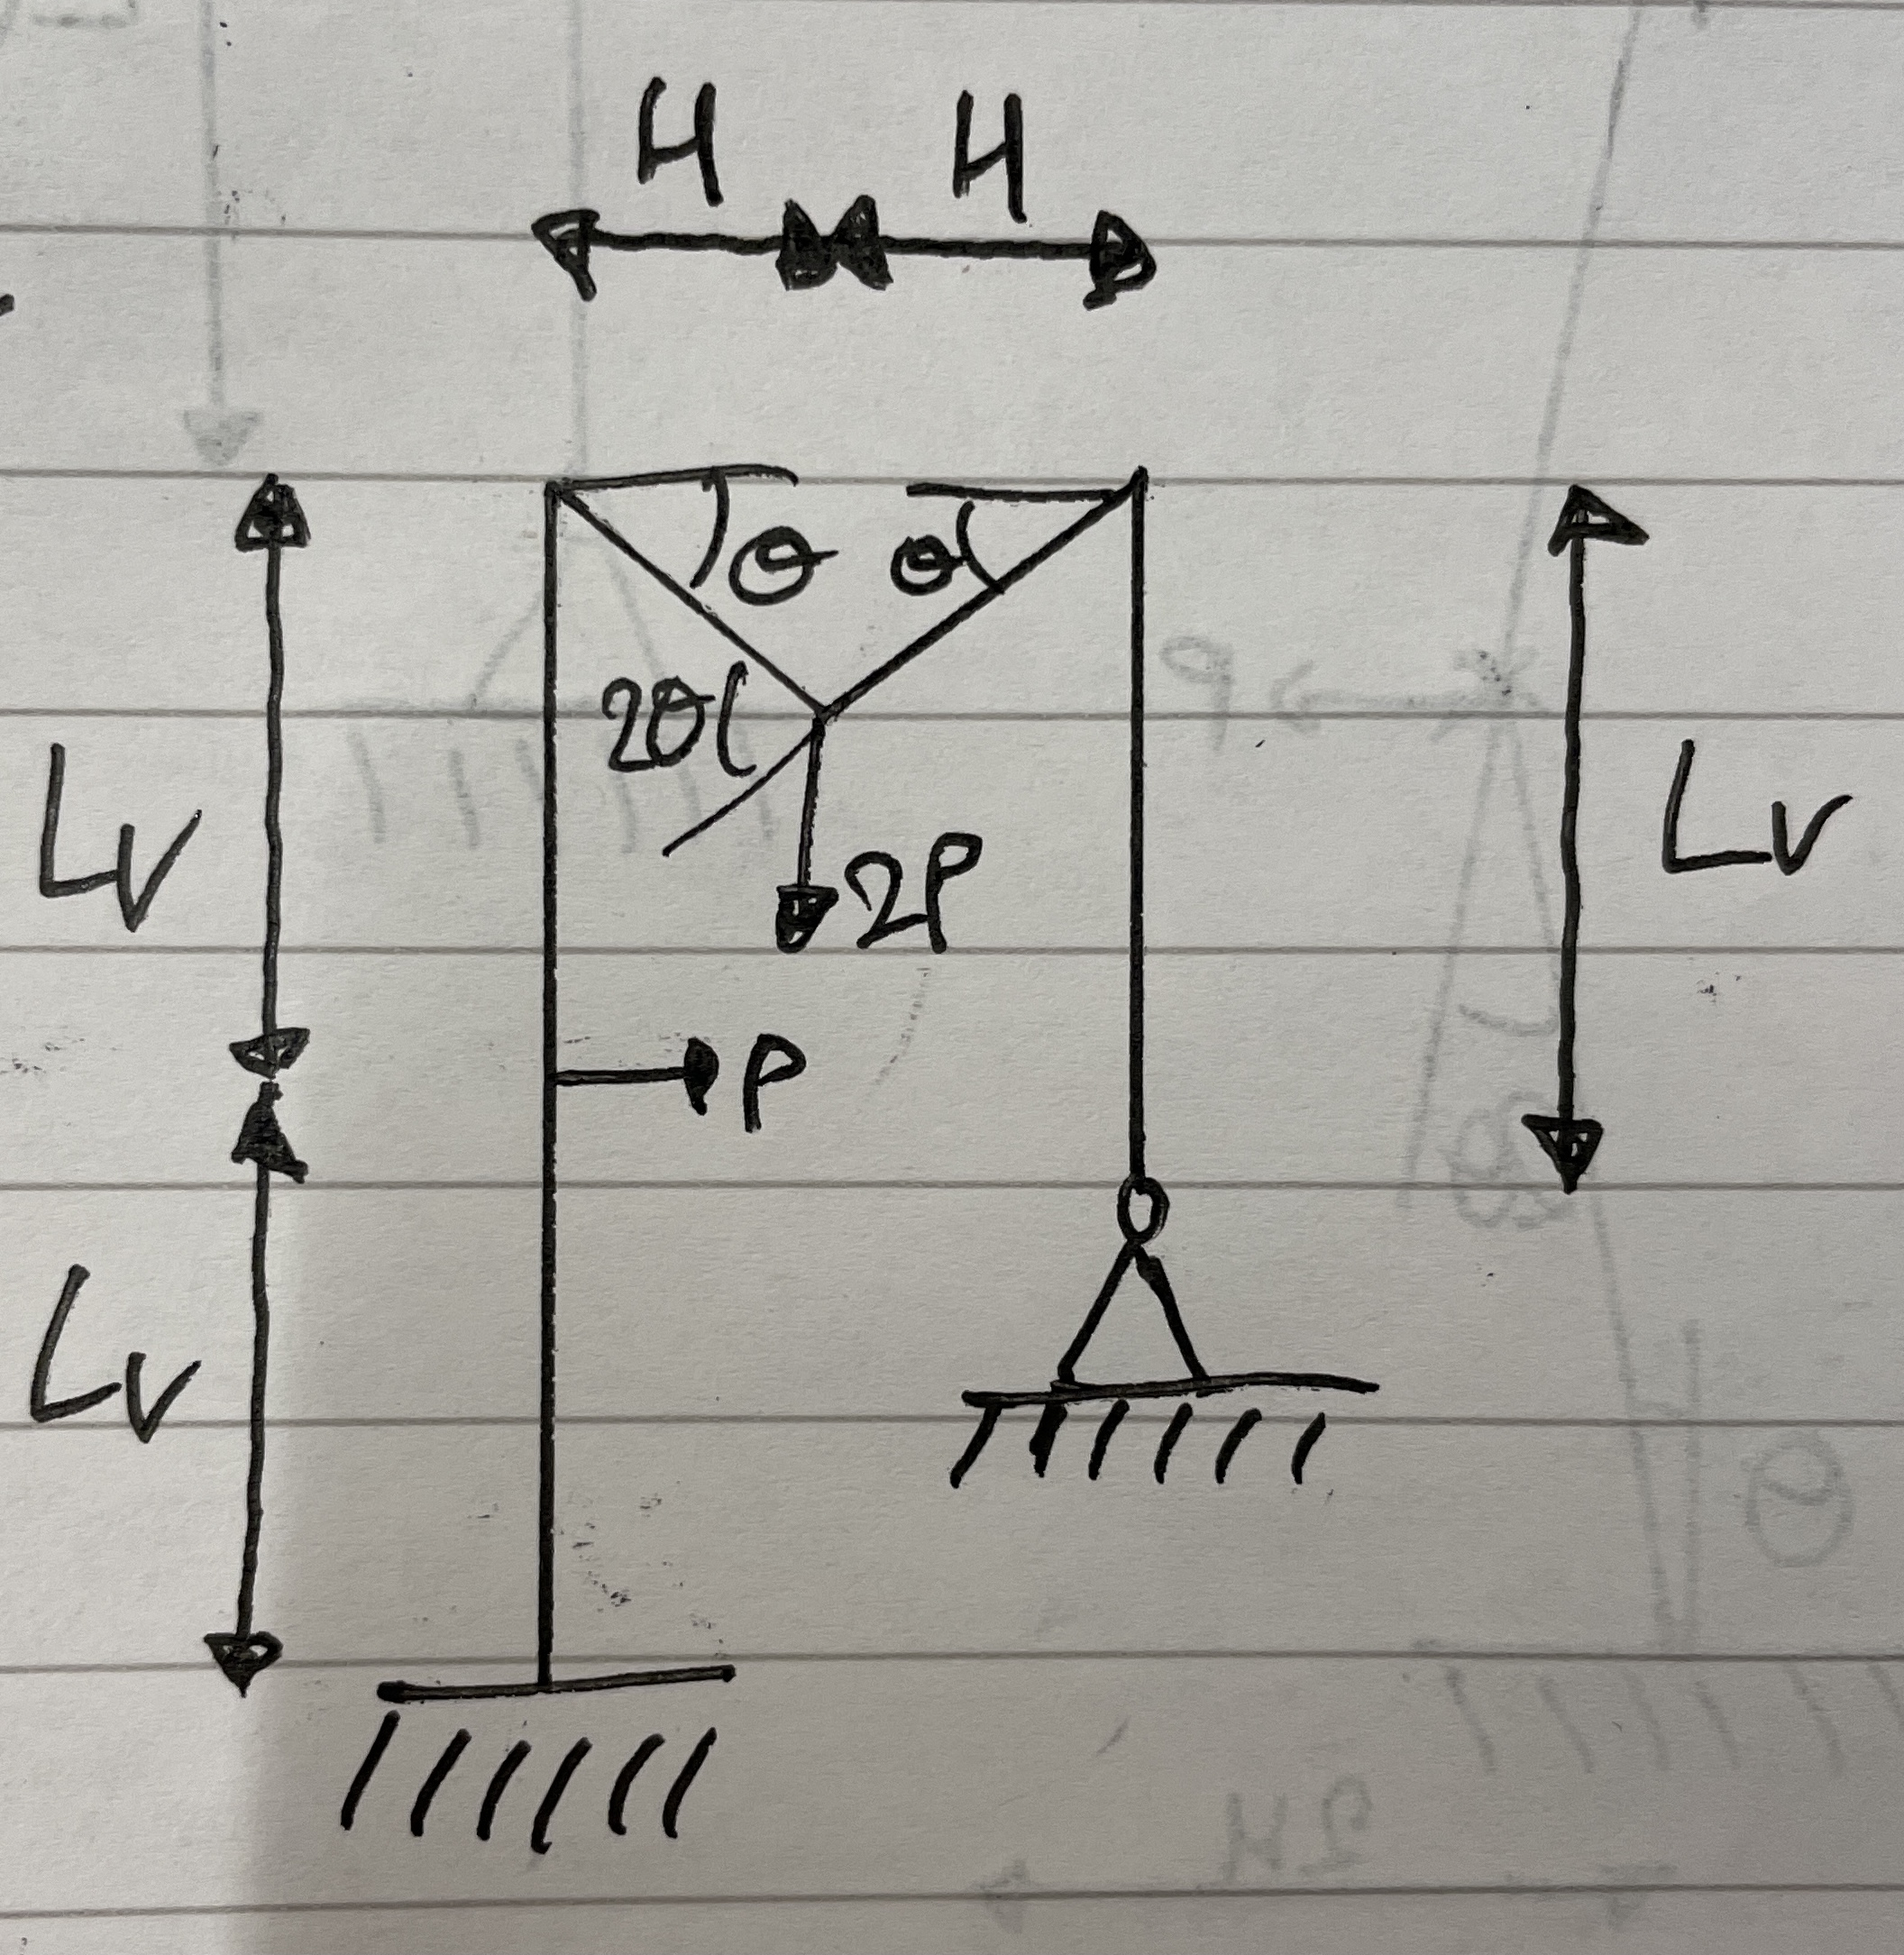
\includegraphics[width = 0.9\textwidth]{./img/q3i2.jpg}
    \caption{Sketch of portal frame undergoing beam collapse.}
\end{figure}
Here, work is done in all the joints on the top beam. 
\begin{align}
    \sum M_P \theta &= \sum Fd\\
    M_P \theta + M_P (2\theta) + M_P \theta &= 2P H \theta\\
    4M_P \theta &= 2PH\theta\\
    P &= \frac{2M_P}{H} 
\end{align}
\begin{figure}[H]
    \centering
    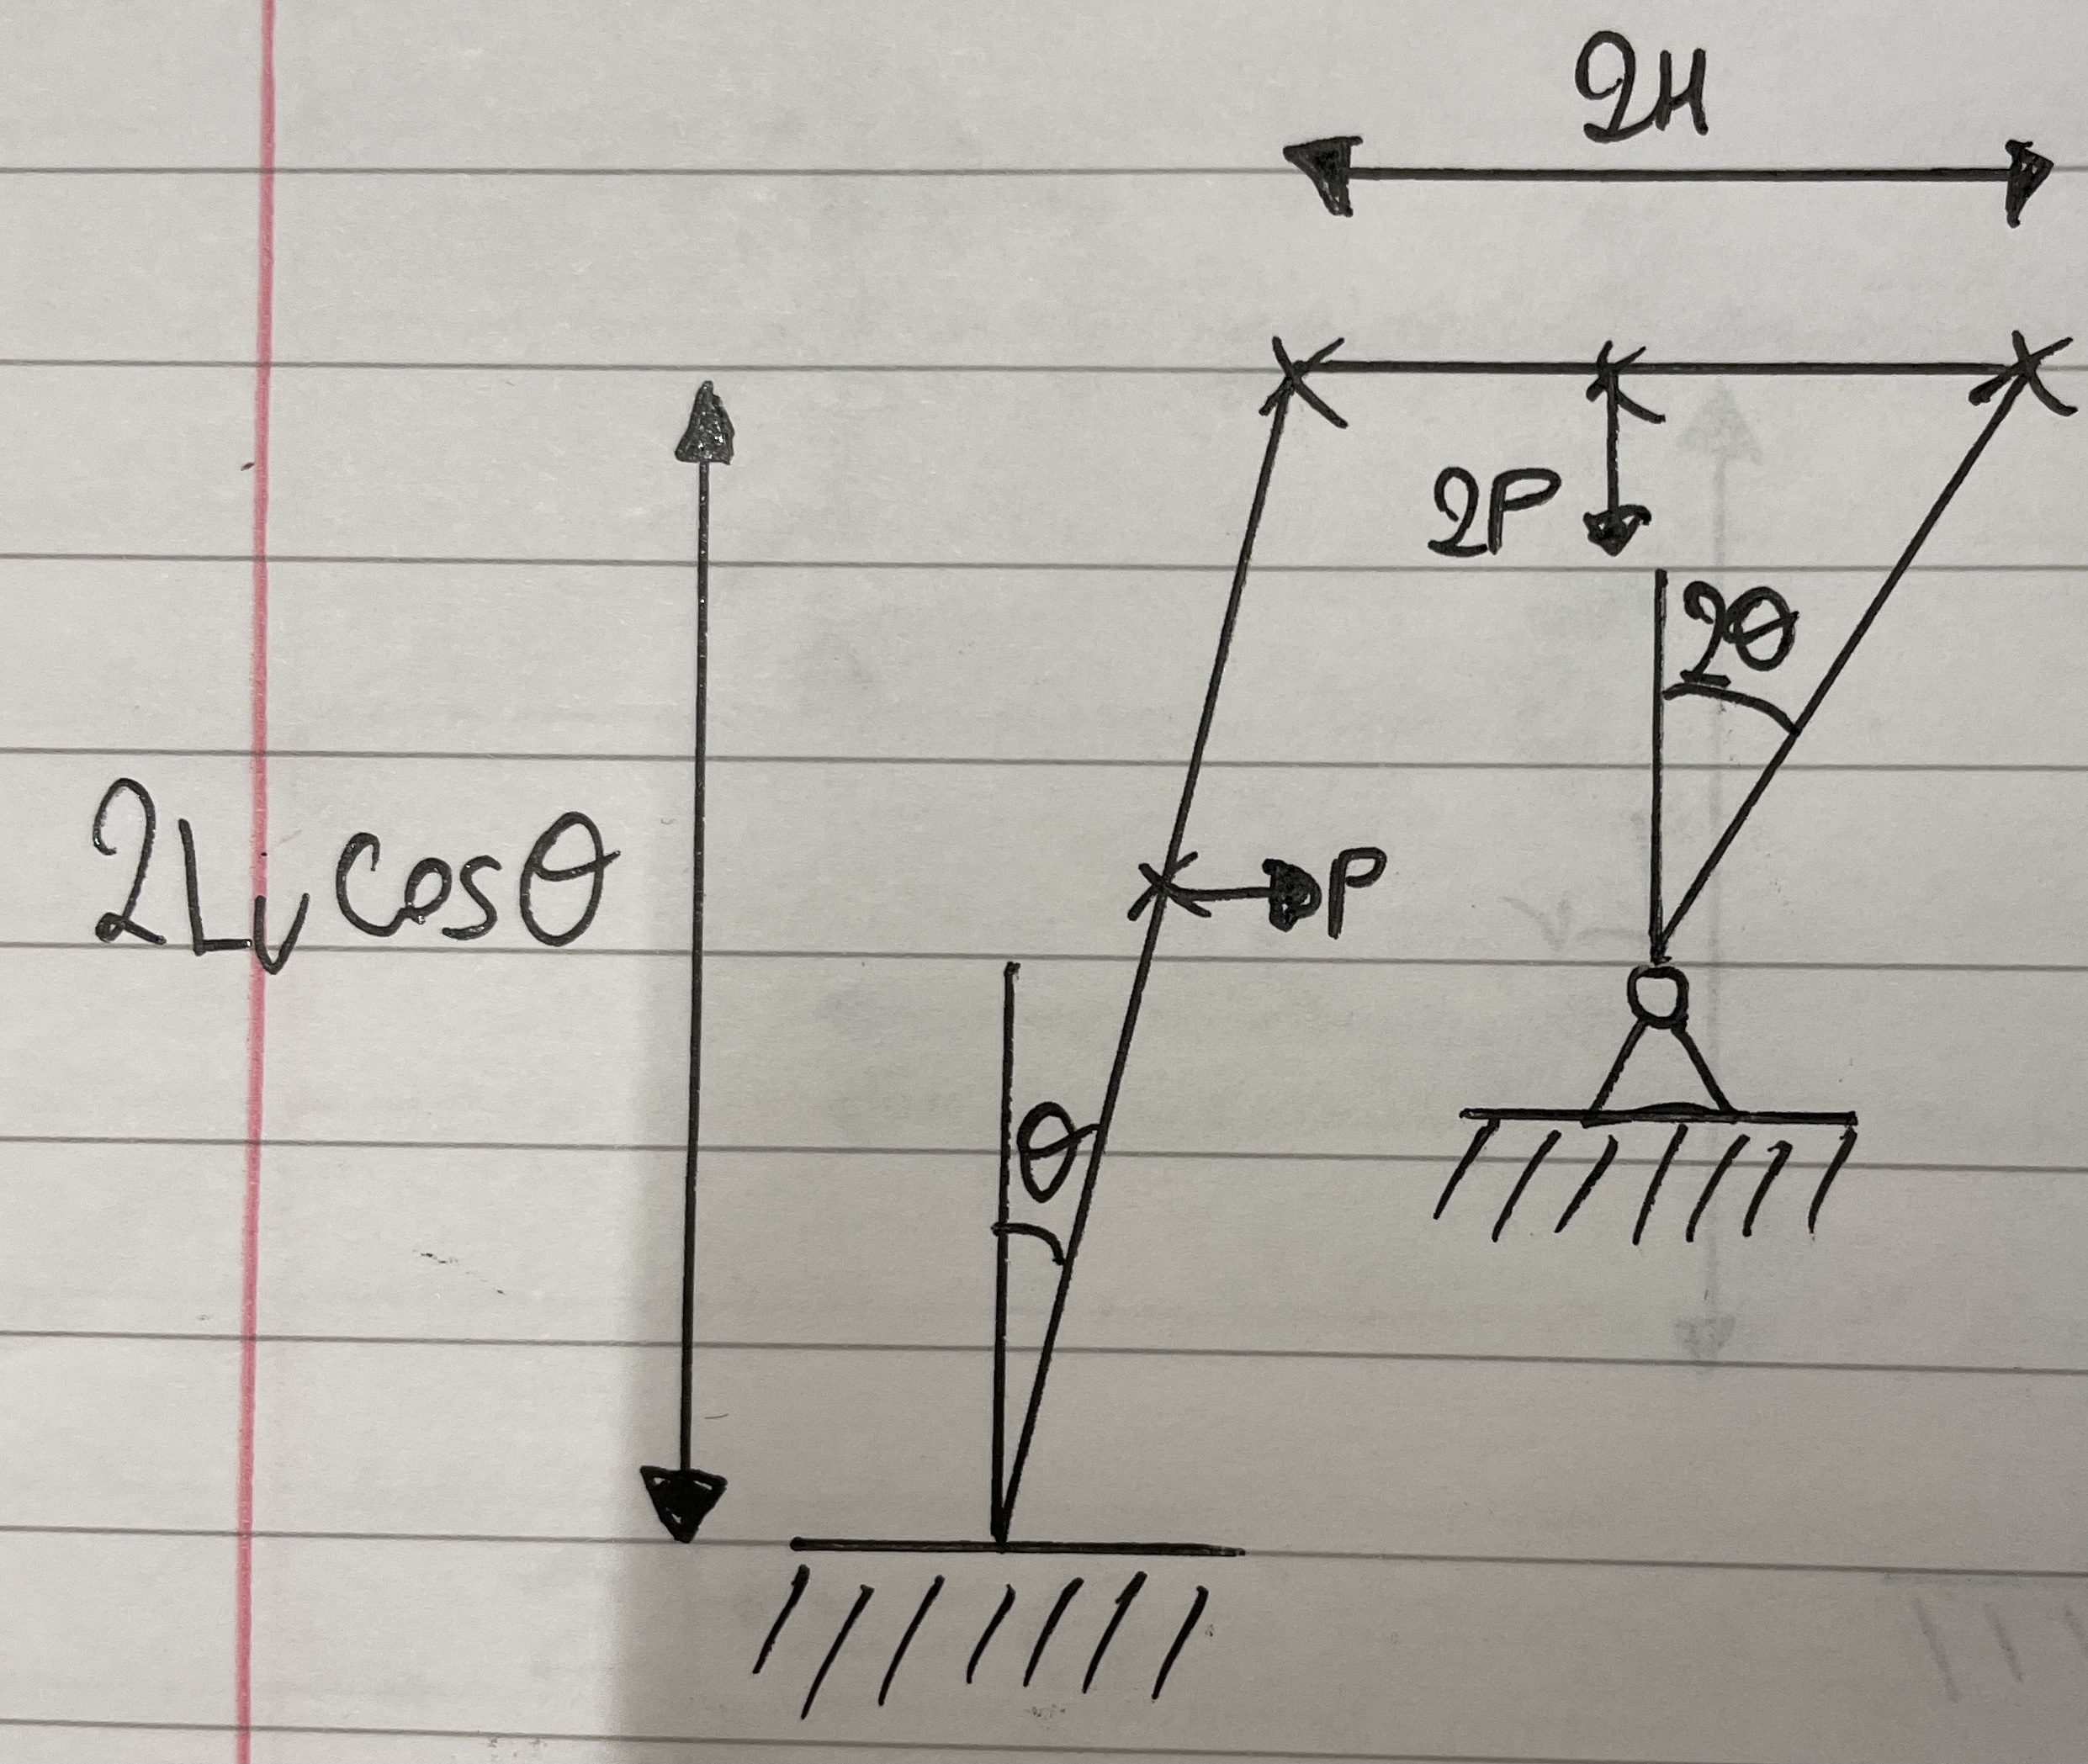
\includegraphics[width =0.9\textwidth]{./img/q3i3.jpg}
    \caption{Sketch of portal frame undergoing sway collapse.}
\end{figure}
Here, work is done at both ends of the long column and at the top end of the short column.
\begin{align}
    \sum M_P \theta &= \sum Fd\\
    M_P\theta + M_P \theta + M_P (2\theta) &= PL_v \theta\\
    4M_P \theta &= PL_v \theta\\
    P &= \frac{4M_P}{L_v}
\end{align}
\begin{figure}[H]
    \centering
    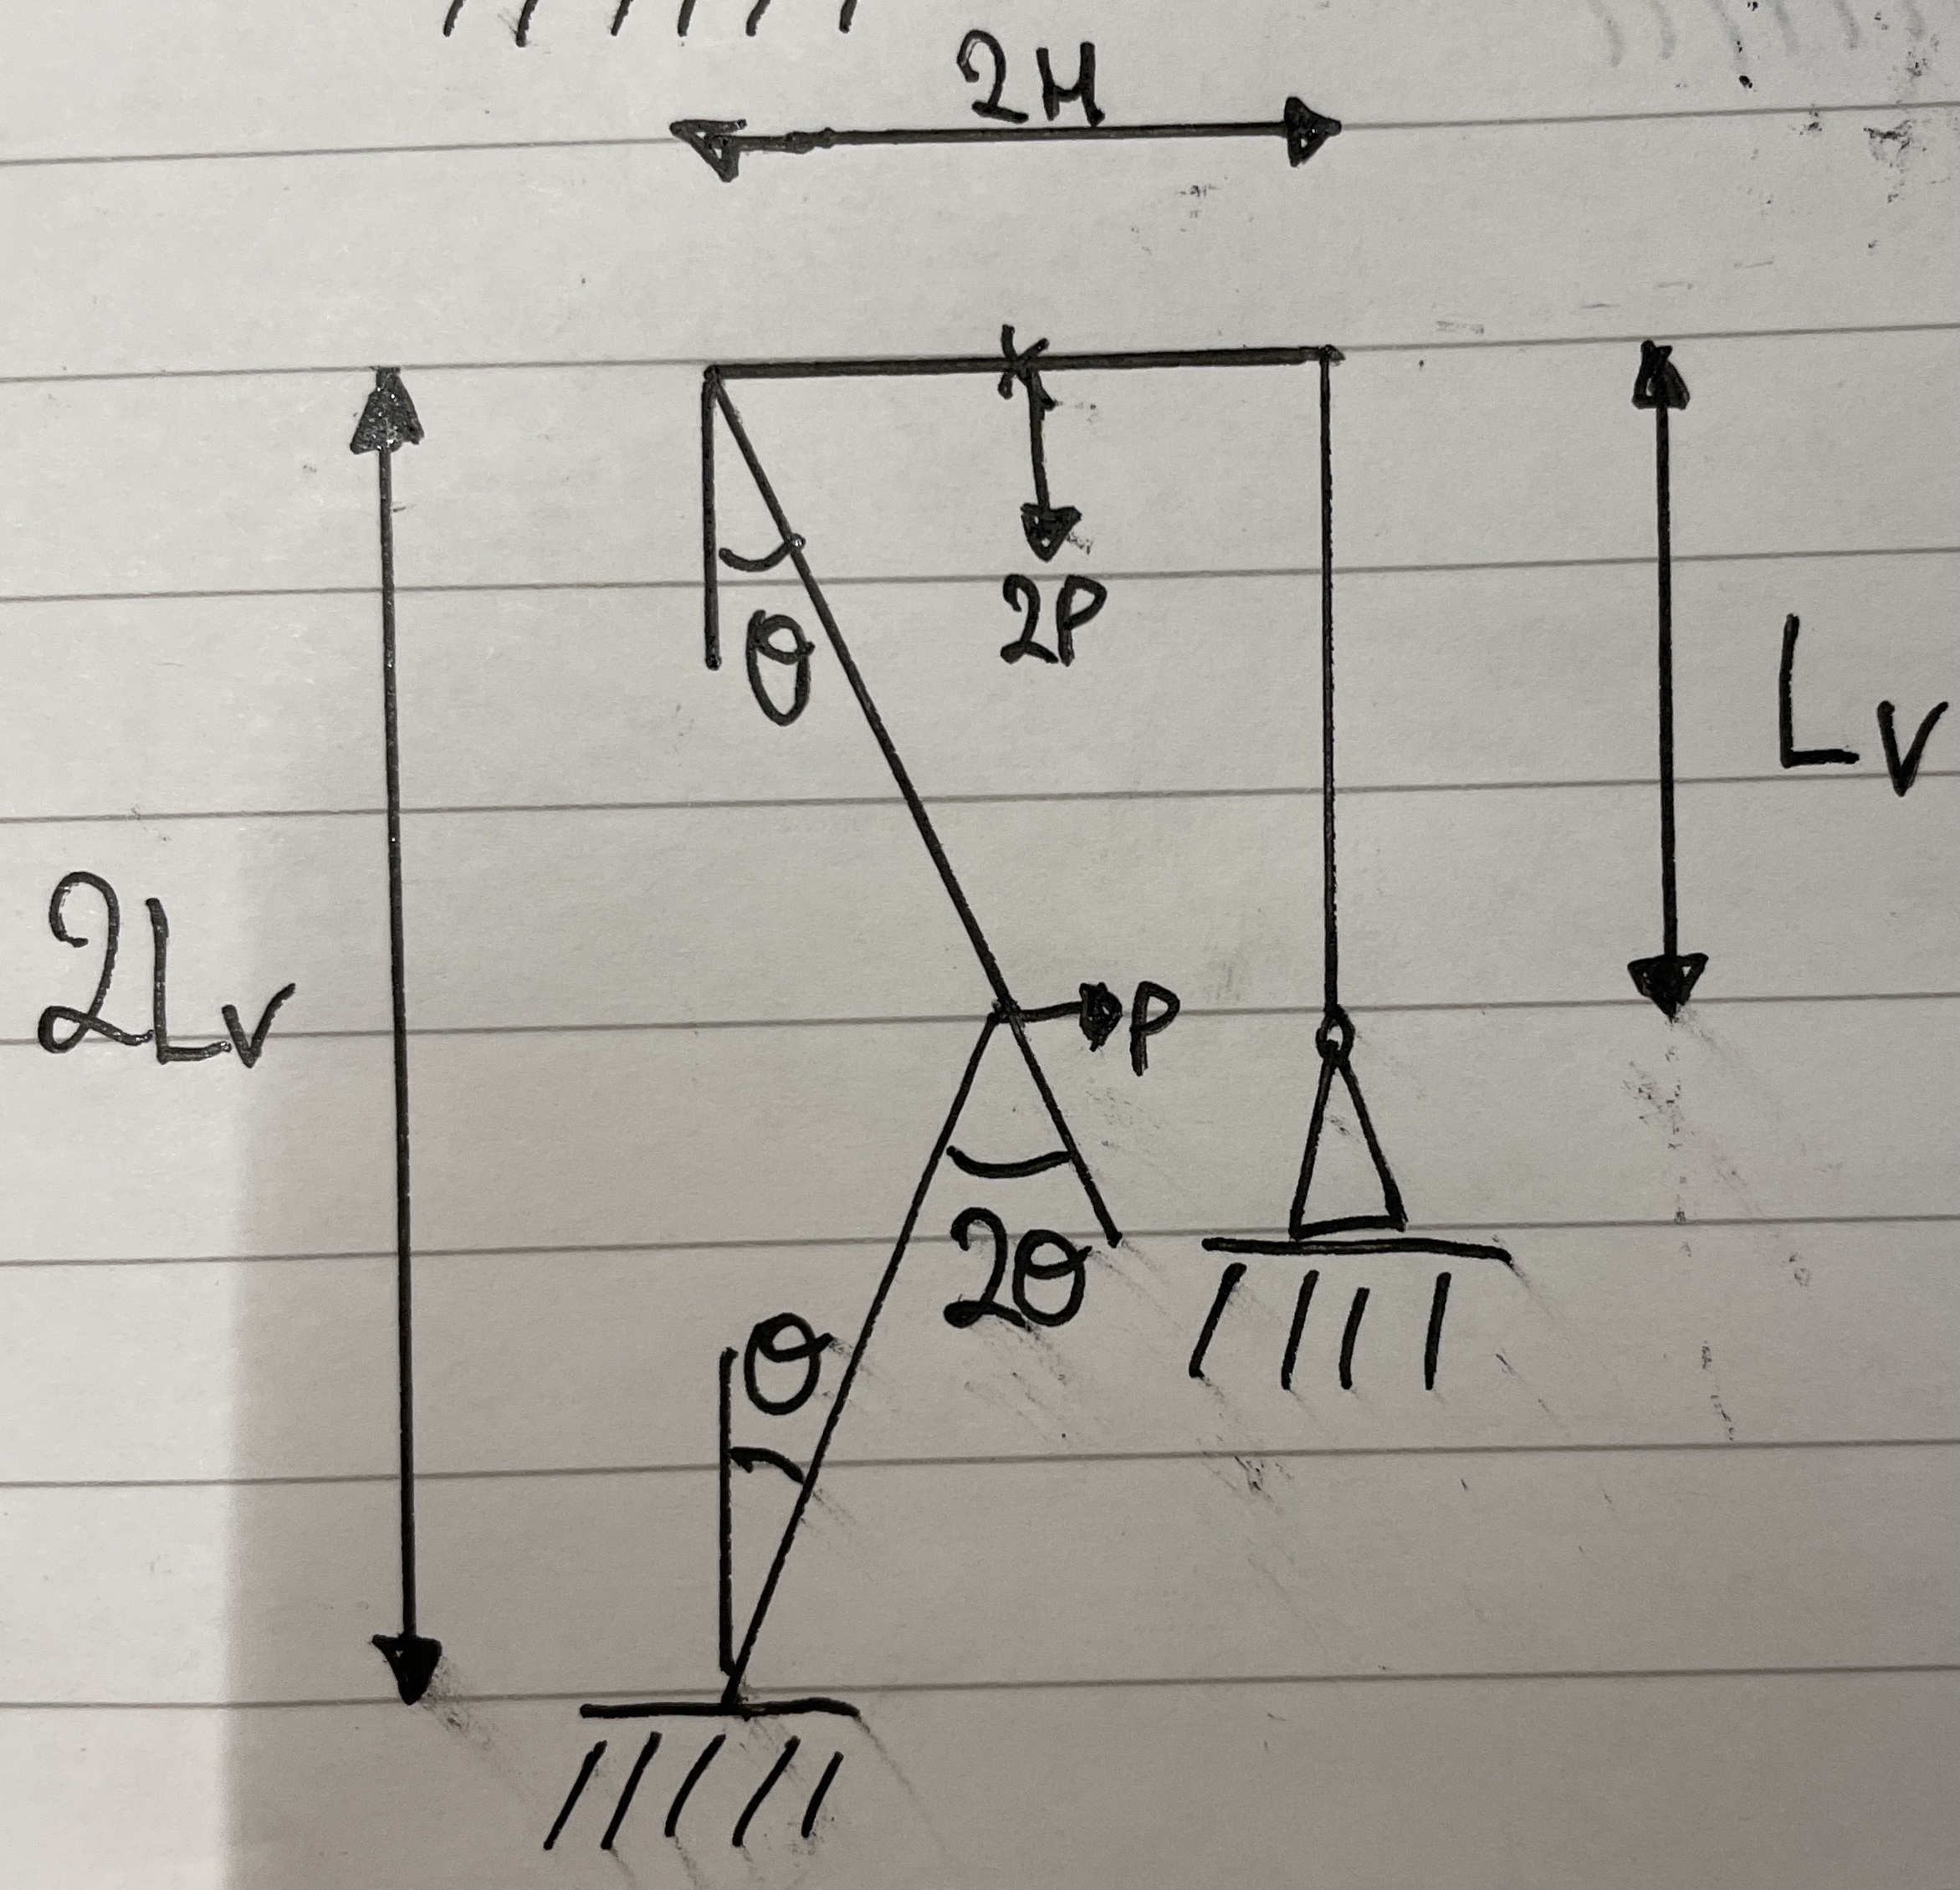
\includegraphics[width = 0.9\textwidth]{./img/q3i5.jpg}
    \caption{Sketch of portal frame undergoing column collapse.}
\end{figure}
Here, work is done at the top, bottom and middle of the long column.
\begin{align}
    \sum M_P \theta &= \sum Fd\\
    M_P \theta + M_P(2\theta) + M_P\theta &= PL_v \theta\\
    4M_P \theta &= PL_v\theta\\
    P &= \frac{4M_P}{L_v}
\end{align}
\begin{figure}[H]
    \centering
    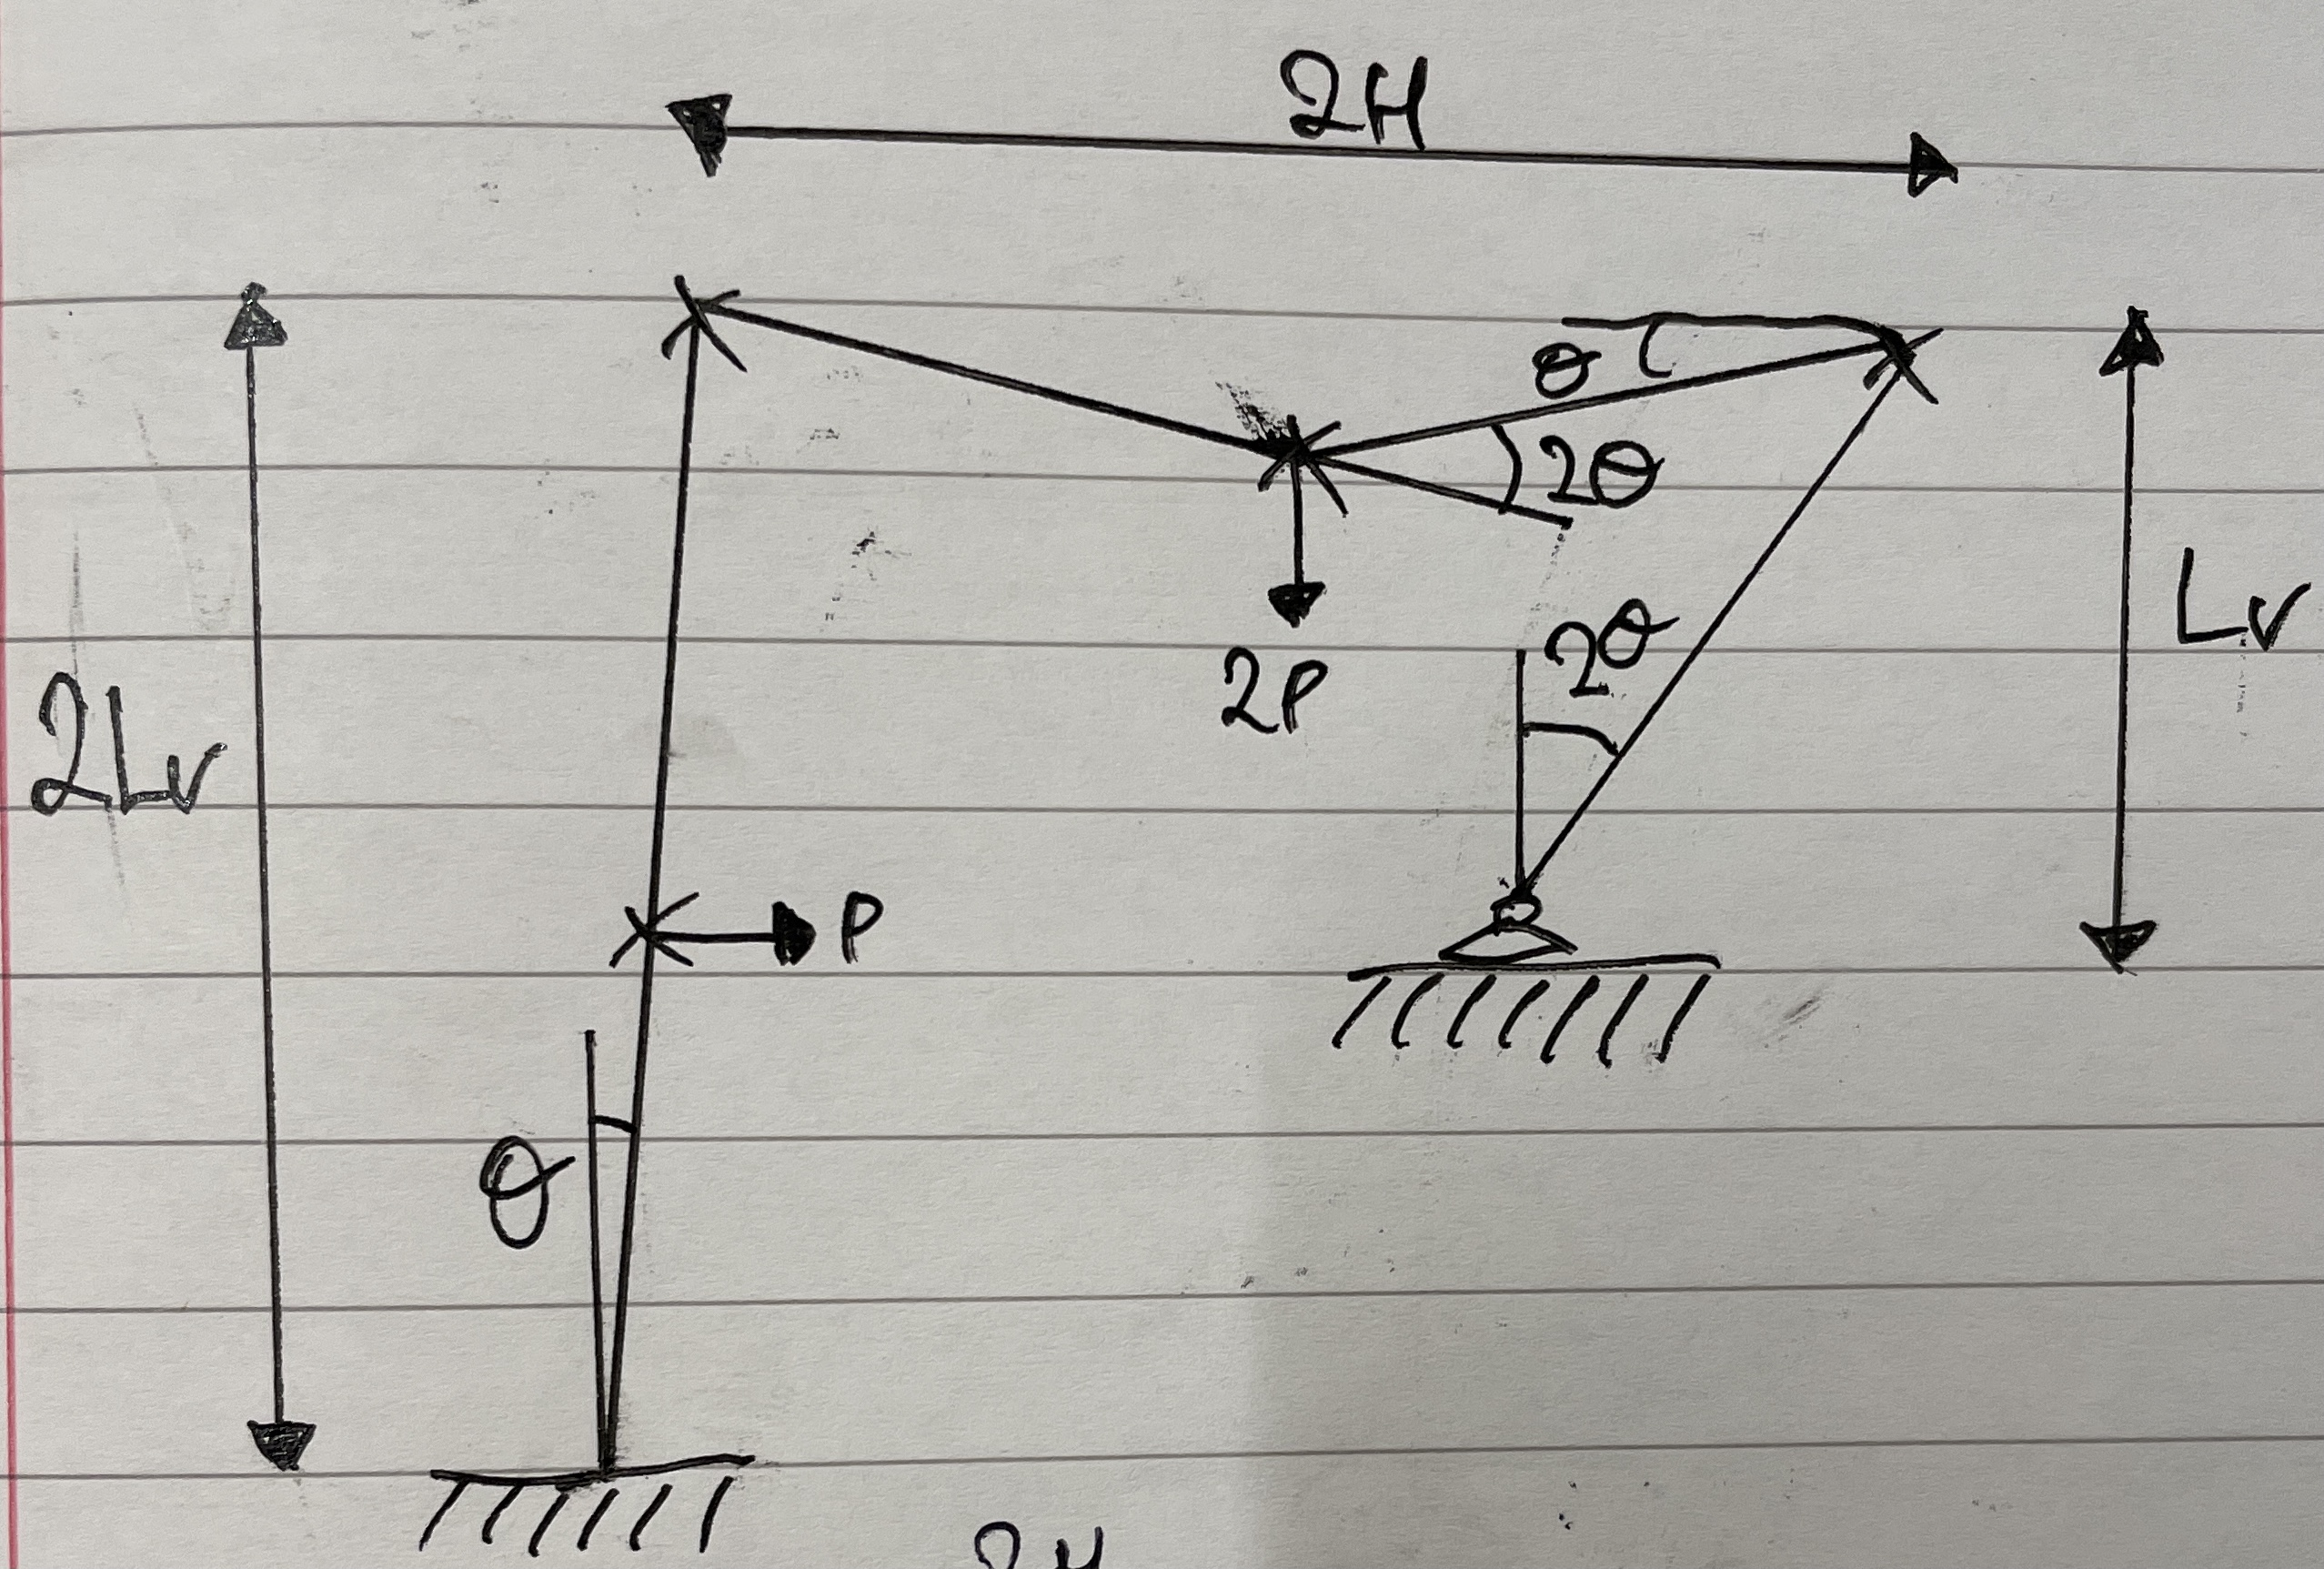
\includegraphics[width = 0.9\textwidth]{./img/q3i6.jpg}
    \caption{Sketch of portal frame undergoing beam and sway collapse.}
\end{figure}
Here, work is done at the base of the long column, the middle of the horizontal beam and the top of the short column. 
\begin{align}
    \sum M_P \theta &= \sum Fd\\
    M_P \theta + M_P (2\theta) + M_P (3\theta) &= 2PH\theta + PL_v\theta\\
    6M_P\theta &= P\theta \left(2H + L_v\right)\\
    P &= \frac{6M_P}{2H + L_v}
\end{align}
\begin{figure}[H]
    \centering
    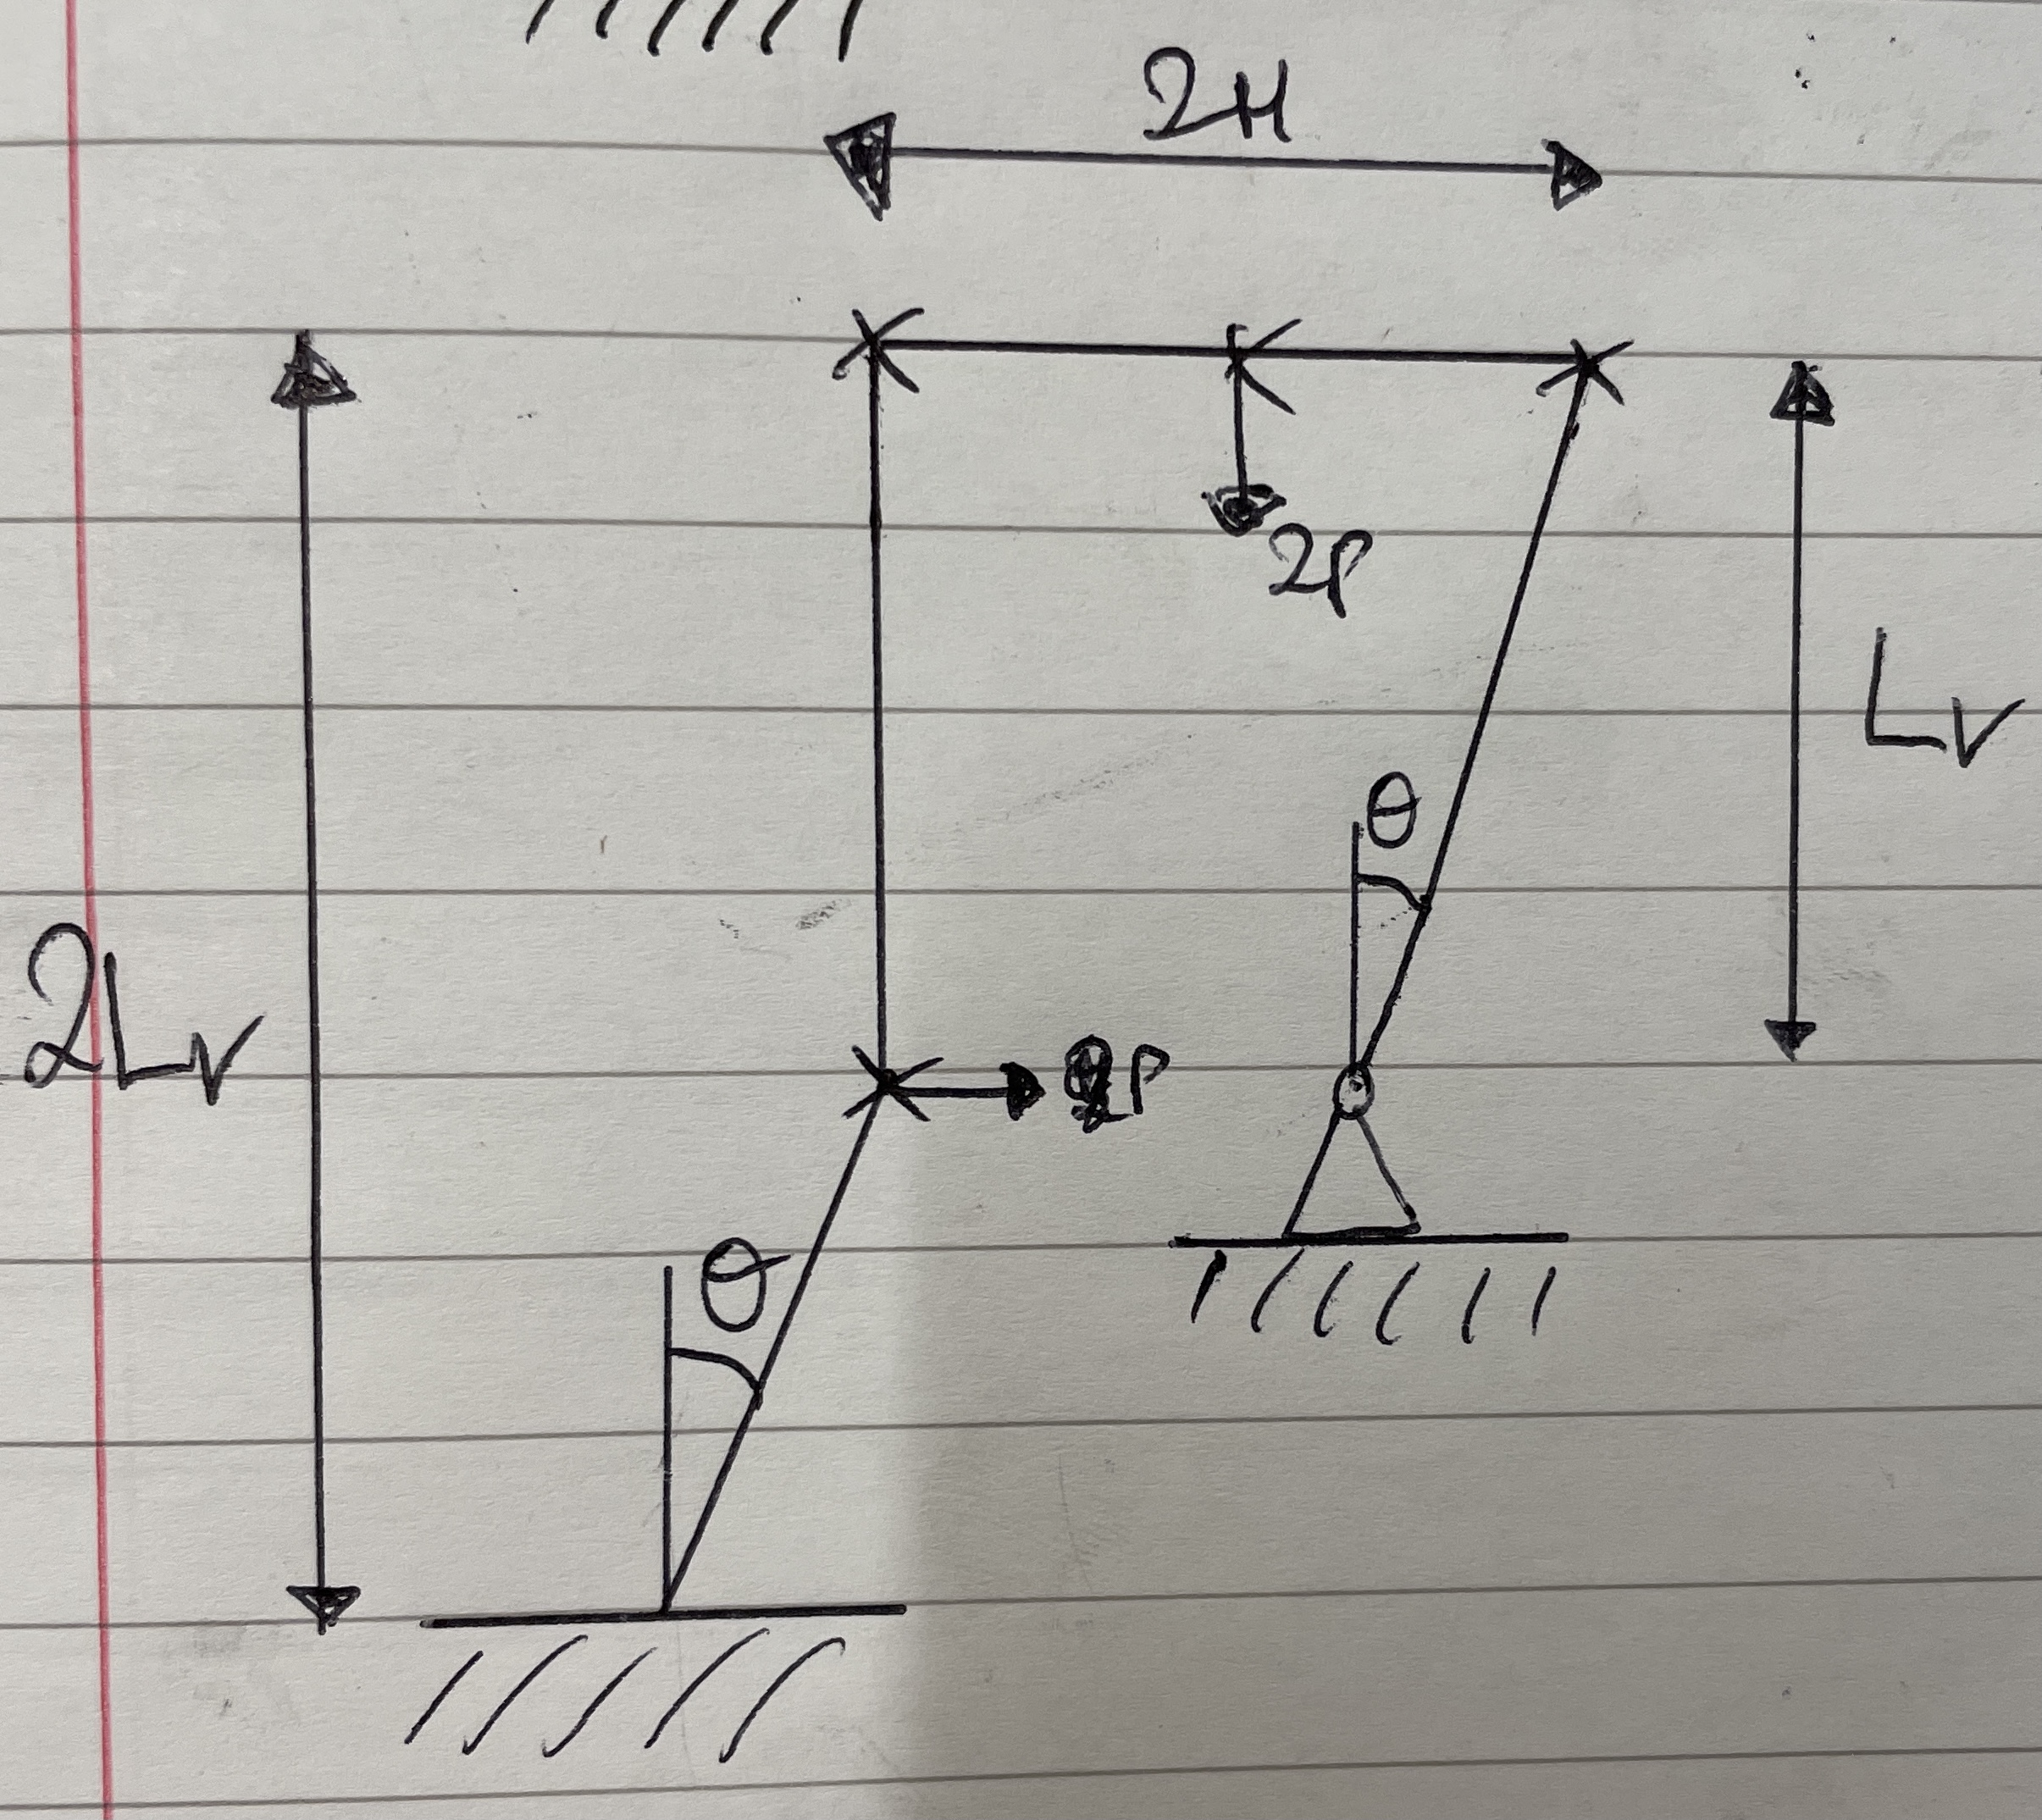
\includegraphics[width = 0.9\textwidth]{./img/q3i7.jpg}
    \caption{Sketch of portal frame undergoing column and sway collapse.}
\end{figure}
Here, work is done at the bottom and middle of the long column, as well as at the top of the short column.
\begin{align}
    \sum M_P\theta &= \sum Fd\\
    M_P\theta + M_P\theta + M_P\theta &= PL_v\theta\\
    3M_P\theta &= PL_v\theta\\
    P &= \frac{3M_P}{L_v}
\end{align}
\subsection{ii}
Let us tabulate our investigations in part i:
\begin{table}[H]
    \centering
    \begin{tabular}{ll}
        \toprule
        Collapse mechanism & Collapse load\\
        \midrule
        Beam collapse & $P = \frac{2M_P}{H}$\\
        Sway collapse & $P = \frac{4M_P}{L_v}$\\
        Column collapse & $P = \frac{4M_P}{L_v}$\\
        Beam and sway collapse & $P = \frac{6M_P}{2H + L_v}$\\
        Column and sway collapse & $P = \frac{3M_P}{L_v}$\\
        \bottomrule
    \end{tabular}
    \caption{Table to show equations of $P$ from possible collapse mechanisms of portal frame.}
    \label{tab:collapses}
\end{table} requested mode of collapse is column and sway. Hence, we must select our $H$ value to ensure that column and sway collapse is the most likely to occur (when certain loading conditions are met). Using $L_v = 0.75$:
\begin{equation}
    P_{cr} = \frac{3M_P}{0.75} = 4 M_P
\end{equation}
Let us check to see if the other collapse mechanisms have a lower $P_{cr}$ value:
\begin{align}
    \textrm{Sway collapse: } P_{cr} &= \frac{4M_P}{0.75} = \frac{16M_P}{3}\\
    \textrm{Column collapse: } P_{cr} &= \frac{4M_P}{0.75} = \frac{16M_P}{3} 
\end{align}
Sway and column collapse have higher $P_{cr}$ values than column and sway collapse. Now we can begin to select a H value. Beam collapse:
\begin{align}
    4M_P &< \frac{2M_P}{H}\\
    H &< 0.5
\end{align}
Beam and sway collapse:
\begin{align}
    4M_P &< \frac{6M_P}{2H + 0.75}\\
    8H + 3 &< 6\\
    H &< 0.375
\end{align}
Hence, we can see that a suitable value of $H$ may be $H < 0.375$. Let us select a value of $H = \SI{0.35}{\meter}$.
\subsection{iii}
We want our collapse to occur at $P_{cr} = \frac{2}{3}P_Y$. $P_Y$ was calculated to be \SI{637}{\newton} in Q1iii. Hence:
\begin{align}
    P_{cr} = \SI{425}{\newton}
\end{align}
Calculating $M_P$:
\begin{align}
    P_{cr} &= \frac{3M_P}{L_v}\\
    425 &= \frac{3M_P}{0.75}\\
    M_P &= \SI{106.25}{\newton\meter}
\end{align}
Next we can check the columns of the portal frame:
\begin{align}
    \frac{2}{3}P_Y &= 4M_P\\
    P_Y &= 6M_P = \frac{3}{2}P_{cr}\\
\end{align}
Left column analysis. We must ensure that our $P_{cr} < S_{cr}$. Since it is a fixed-fixed column, $L_e = 0.5L$:
\begin{align}
    P_{cr} &< \frac{n^2 \pi^2 E I}{L_e^2}\\
    425 &< \frac{1 \times \pi^2 \times 71 \times 10^9 \times I}{0.75^2}\\
    I &> \SI{3.41e-10}{\meter\tothe{4}} \textrm{ (3sf)}
\end{align}
Right column analysis. We must ensure that our $P_{cr} < S_{cr}$. Since it is a pinned-fixed column, $L_e = 0.7L$:
\begin{align}
    P_{cr} &< \frac{n^2 \pi^2 E I}{L_e^2}\\
    425 &< \frac{1 \times \pi^2 \times 71 \times 10^9 \times I}{(0.7\times 0.75)^2}\\
    I &> \SI{1.67e-10}{\meter\tothe{4}} \textrm{ (3sf)}
\end{align}
Our second moment of area must be greater than I $>$ \SI{3.41e-10}{\meter\tothe{4}}.
\begin{figure}[H]
    \centering
    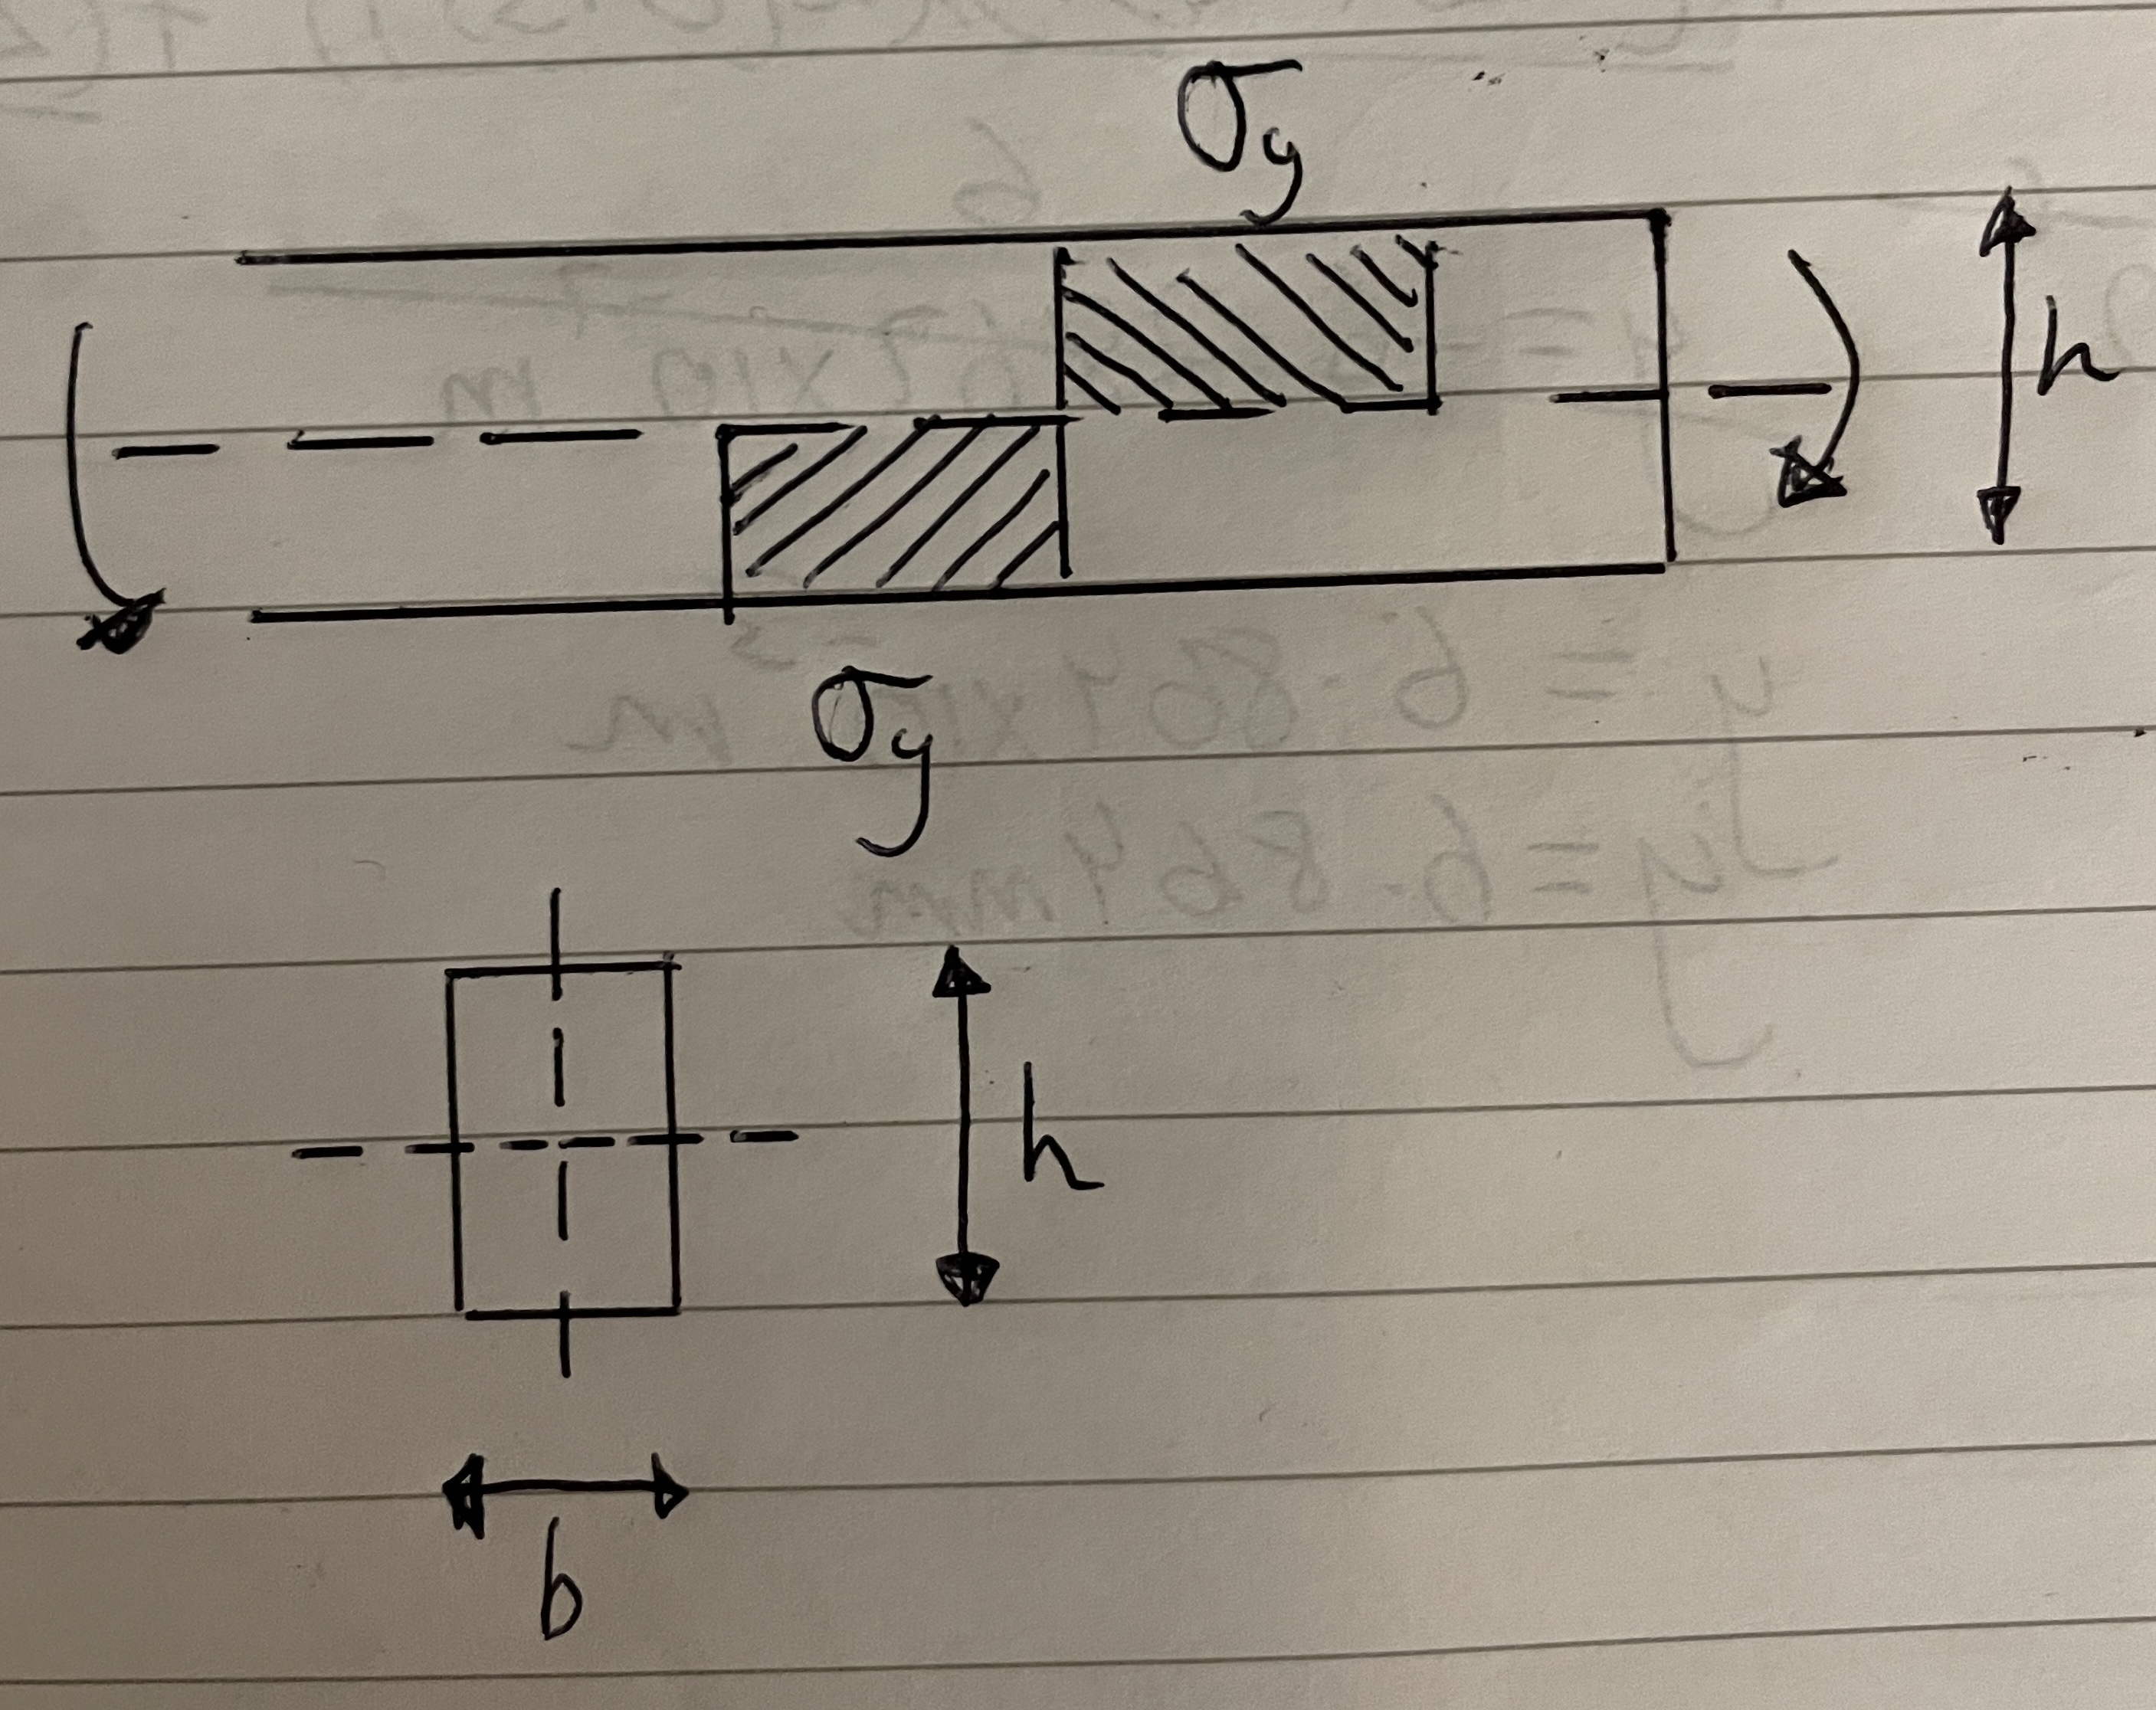
\includegraphics[height = 7cm]{./img/q3iii1.jpg}
    \caption{Sketch of portal frame undergoing column collapse.}
\end{figure}
Calculating the plastic bending moment:
\begin{align}
    M_P &= \sigma_Y \frac{bh^2}{4}\\
    106.25 &= (186\times 10^6)\frac{bh^2}{4}\\
    bh^2 &= \SI{2.28e-6}{\meter^3}
\end{align}
Selecting a value of $b = \SI{0.01}{\meter}$:
\begin{align}
    h &= \sqrt{\frac{2.28\times 10^6}{0.01}}\\
    h &= \SI{0.0151}{\meter}
\end{align}
Now we can calculate our second moment of area and compare this to the limiting value we found earlier. 
\begin{align}
    I &= \frac{bh^3}{12}\\
    I &= \frac{0.01 \times 0.0151^3}{12}\\
    I &= \SI{2.87}{\meter\tothe{4}}
\end{align}
\SI{2.87}{\meter\tothe{4}} $>$ \SI{3.41e-10}{\meter\tothe{4}}, hence $P_{cr} < S_{cr}$ is satisfied for both columns and design is suitable. 
\begin{align}
    M_P &= (186\times 10^6)\frac{0.01 \times 0.0151^2}{4} = \SI{106}{\newton \meter} \textrm{ (3sf)}
\end{align}
The cross-section satisfies that $P_C = \frac{2}{3} P_Y$. 
\end{document}